\documentclass[12pt, a4paper,twoside]{report}
	
	\usepackage{comment}
	\usepackage{mathtools,amsthm} % Enable useful mathematical symbols/environments
	\usepackage{graphicx} % Enable graphics
	\usepackage{fancyhdr,titlesec,microtype} % enable various formatting commands
	\usepackage[margin=2.5cm]{geometry} % Set margin size
	\usepackage{merriweather} % Set the font
	\usepackage[latin1]{inputenc} % Allow you to input accents, umlauts and other characters
	\usepackage[T1]{fontenc} % Lets LaTeX print a wider array of characters
	\usepackage{tablefootnote}
	\usepackage[most]{tcolorbox}
	\usepackage{xcolor} % Enable coloured elements
	\definecolor{mypurple}{HTML}{622567} %%% Purple
	\definecolor{primaryc}{HTML}{8f5e77} %%%EssexOrange
	\definecolor{myblue}{HTML}{007A87} %%%Seagrass
	\usepackage{footnotehyper}
	\usepackage{caption}
	% For technical reasons, hyperref should be loaded after all other packages
	\usepackage[colorlinks,linkcolor=myblue,citecolor=mypurple, urlcolor=myblue]{hyperref}
	
	\renewcommand{\baselinestretch}{1.5} % 1.5 line spacing
	
	% Define \begin{theorem}, \end{theorem}, etc.
	\theoremstyle{plain} % The following will be italicised
	\newtheorem{theorem}{Theorem}[chapter]
	\newtheorem{lemma}[theorem]{Lemma}
	\newtheorem{proposition}[theorem]{Proposition}
	\newtheorem{corollary}[theorem]{Corollary}
	
	\theoremstyle{definition} % The following environments will not use italics
	\newtheorem{definition}[theorem]{Definition}
	\newtheorem{example}[theorem]{Example}
	
	\theoremstyle{remark} % The following environments will not use italics or bold titles
	\newtheorem{remark}[theorem]{Remark}
	
	\numberwithin{equation}{chapter}
	
	\addtolength{\skip\footins}{4pc plus 5pt}
	\setlength{\footnotesep}{1.22\footnotesep}
	
	% Fancy headings
	\pagestyle{fancy}
	\setlength{\headheight}{15pt}
	\fancyheadoffset[LE,RO]{0pt}
	\renewcommand{\chaptermark}[1]{\markboth{#1}{}}
	\renewcommand{\sectionmark}[1]{\markright{\thesection\ #1}}
	\fancyhf{}
	\fancyhead[LE]{\makebox[0pt][l]{\thepage}\hfill\leftmark}
	\fancyhead[RO]{\rightmark\hfill\makebox[0pt][r]{\thepage}}
	\fancypagestyle{plain}{%
		\fancyhead{} % get rid of headers
		\renewcommand{\headrulewidth}{0pt} % and the line
	}
	
	% Fancy  numbers
	\titleformat{\chapter}[display]
	{\normalfont\bfseries\color{primaryc}}
	{\filleft\hspace*{-60pt}%
		\rotatebox[origin=c]{90}{%
			\normalfont\color{black}\Large%
			\textls[180]{\textsc{Section}}%
		}
		\hspace{10pt}%
		{\setlength\fboxsep{0pt}%
			\colorbox{primaryc}{\parbox[c][3cm][c]{2.5cm}{%
					\centering\color{white}\fontsize{80}{90}\selectfont\thechapter}%
			}
		}
	}
	{10pt}
	{\titlerule[2.5pt]\vskip3pt\titlerule\vskip4pt\LARGE\sffamily}
	
	\begin{document} % Start your document
		
		%%%%%%%%%%%% BEGIN TITLE PAGE %%%%%%%%%%%%
		
		\thispagestyle{empty} % For the title page, no header / footer
		
		\noindent
		\begin{minipage}{0.1\textwidth}
		\end{minipage}
		\hfill
		
		\begin{center}
			\noindent\textcolor{primaryc}{\rule{\linewidth}{4.8pt}}
			
			\vspace{2em}
			
			\vspace{3em}
			\noindent {\Huge{\color{myblue} Claims Denials In U.S. Health Insurance}}
			
			\vspace{3em}
			{\small \today }
			\begin{comment}
				\noindent {\Large \bf Mike Gartner}
			\end{comment}
			\vfill
			Claims denials in U.S. health insurance pose a serious problem for consumers navigating their care. In this report we present and analyze data that sheds light on the occurrence and prevalence of claims denials, propose policies to improve patient outcomes, and highlight existing avenues for consumer recourse.
			\vfill
			

			
			\vspace{0.5em}
			\noindent\textcolor{primaryc}{\rule{\linewidth}{4.8pt}}
			

			
			\vspace{3em}
			
\includegraphics[width = 10mm]{images/persius/favicon.png}
			\hspace{2mm}
			
\includegraphics[width = 50mm]{images/persius/persius_f1_maroon.png}\\[8ex]
		\end{center}
		
		\clearpage
		
		%%%%%%%%%%%% END TITLE PAGE %%%%%%%%%%%%
		
		\tableofcontents
		
		% If you have lots of figures with captions / numbers, uncomment the following line
		%\listoffigures
		
		% If you have lots of tables and want a list of them, uncomment the following line
		%\listoftables
		
		\chapter{Introduction}\label{intro}
		
		\hspace{2em} Claims are a fundamental and atomic unit of U.S. health insurance: every time an insured consumer attempts to use their health insurance to cover a portion of a bill, a claim is submitted to their insurer on their behalf. The claim records details about the care received and its cost necessary for an insurer to make a payment determination. The primary role of health insurers is to receive and adjudicate these claims based on the contracts they sell, and ultimately pay for some portion of them, on behalf of those who purchased the contracts (typically employers or individuals).\\
		
		When insurers adjudicate a claim to determine whether they will pay for it, they review the contracts that govern the coverage which has been purchased on behalf of the insured. The permissible content in these contracts is often restricted by various laws and regulations, and the contracts may also refer to external sources (e.g. "clinical policy bulletins", or "scientific literature") that are explicitly cited as things that will be used to inform coverage determinations. We will say a coverage decision or denial is contractually inappropriate if the decision is inconsistent with the insurance contract governing a policy, or the laws and regulations that apply to that policy.\\
		
		We note that there are many coverage decisions that one might deem morally or medically inappropriate that would not be considered contractually inappropriate. For example, it would be morally troubling for corporations to sell policies that opaquely exclude the coverage of commonly used, scientifically proven, but expensive treatments for those facing dire medical situations, and then to enforce those exclusions no matter the extenuating or dire circumstances. However, such behavior is, unfortunately, not necessarily contractually inappropriate or illegal, depending on the contract in question.\\
		
		The prevalence of contractually inappropriate claims denials, and lack of recourse for consumers even in these cases, have been serious problems for a long time. There are organizations that regularly publish reports analyzing the limited publicly available claims denial data \cite{pollitz2021} that point to this prevalence (e.g. when comparing appeal rates to appeal overturn rates), and the subject has been discussed in policy research, legal research \cite{fox2022} and popular journalism \cite{konrad2010} for a long time.\\
		
		Recently, there have been numerous investigations and articles that have brought to light for the general public just how damaging some of the inappropriate practices taking place really are \cite{armstrong2023a} \cite{armstrong2023b}, and illuminated the scarcity of publicly available data \cite{fields2023}. Finally, there are those most seriously affected; many patients with dire, serious, or chronic medical needs (and their friends and families) have long known about the lack of recourse they enjoy, and the frequency with which contractually inappropriate denials occur just in seeking their own care -- they have been on the front lines for decades, suffering the consequences of an inadequately regulated industry.\\
		
		
		\chapter{A Primer On Claims Denials}\label{primer}
		
		\hspace{2em} A \emph{claim denial} occurs when a claim is submitted to an insurer, and the insurer decides they will not pay for it. In practice, such decisions are made for many reasons; some valid \footnote{\emph{Valid} here could mean medically, morally or contractually valid. We again note that these notions of validity are rarely the same. We will always explicitly qualify the words appropriate or valid if we are specifically referring to a particular notion.}, and others inappropriate or indefensible.\\
		
		When a claim is denied, a patient is typically left with an out of pocket expense larger than what they would otherwise face.

		\subsection{Denials}
		
		\hspace{2em} One of the most basic metrics that one can use to investigate how claims handling varies is an overall \emph{claims denial rate}. This measures the fraction all claims submitted that are denied:
		
		\begin{equation*}
			\text{Denial Rate} = \dfrac{\text{Claims Denied}}{\text{Claims Received}}
		\end{equation*}
		\hfill\\
		In fact, this is not a uniquely defined notion, because the numerator and denominator can be defined in various ways. For example, one could compute this ratio for all claims submitted to a particular insurer over the course of a year, or for all of the claims submitted for a particular plan over a month, or even for all claims submitted from just one individual to a given plan over the course of a year \footnote{Trying to estimate this last number when choosing an insurer is particularly important for individuals with serious health needs who would be unable to afford the care they need if it were to get denied by their insurer.}. We will calculate denial rates that fit this form from a few different lenses in what follows.\\
		
		It is worth noting that:
		
		\begin{enumerate}
			\item \emph{Among the claims that are appropriate}, low denial rate is always a good thing for patients. \footnote{Of course not all claims are actually appropriate. For example, sometimes two duplicate claims are submitted for the same care (administratively inappropriate), and approving such claims would in no way help patients. }.
			\item High denial rates can be caused by numerous things, and do not always indicate \emph{contractually inappropriate} insurer practices.
		\end{enumerate}
		
		
		\subsection{Appeals}
		
		When insurers deny claims, patients are often entitled to an appeals process (e.g. those with federal marketplace plans \href{https://www.healthcare.gov/appeal-insurance-company-decision/appeals/}{are afforded such recourse}, as are all others with so-called \emph{non-grandfathered} qualified health plans; see \cite{pollitz2021} for more background).\\
		
		The details of these processes vary based on details of ones insurance plan, but typically they allow patients to initially file an internal appeal of the denial, which is adjudicated by the insurer themselves. If the internal appeal process (which in some plans requires two attempts at an internal appeal) results in the insurer upholding their denial, patients are then often able to file an external appeal. This means they can submit an appeal of the decision to a (purportedly unbiased \footnote{While we do not have evidence to suggest these organizations make determinations in ways biased towards favorable insurer outcomes, we maintain a healthy dose of skepticism about the independence of their decisions, given the landscape of perverse incentives plaguing the entire space. For example, it is unclear to what extent employees migrate between insurance companies and external review agencies. We invite regulators and lawmakers to publish more data publicly supporting the independence and unbiased nature of such agencies. Lack of public consumer access to detailed denial data, including e.g. determination patterns and methodologies among different review agencies, inspires distrust in a system alread plagued by injustices.}) third party, who is responsible for weighing on the decision; insurers are then legally obligated to uphold the final determinations of these third parties. The third parties, and processes by which external appeals are submitted to them and reviewed by them, vary by plan and by state.\\
		
		In understanding the landscape of claims denials, it is useful to understand the frequency of occurrence, and distribution of outcomes, of these appeal processes.\\
		
		\subsubsection{Initial Appeal Rates}
		
		We define the \emph{internal appeal rate} to be the fraction of denied claims that are appealed at the lowest level available to consumers.\\
		
		\begin{equation*}
			\text{Internal Appeal Rate} = \dfrac{\text{Claims Appealed (@ first level)}}{\text{Claims Denied}}
		\end{equation*}
		\hfill\\
		
		Again, this is a loose definition that we will specify more precisely in each particular calculation below.\\
		
		Of those denials that are internally appealed, we denote the fraction that are overturned by the insurer as the \emph{internal appeal overturn rate}.\\
		
		\begin{equation*}
			\text{Internal Appeal Overturn Rate} = \dfrac{\text{Claims Overturned (@ first level)}}{\text{Claims Appealed (@ first level)}}
		\end{equation*}
		\hfill\\
		
		
		\subsubsection{External Appeal Rates}
		
		We define the \emph{external appeal rate} to be the fraction of internally appealed and subsequently upheld denials which are then additionally externally appealed by consumers.\\
		
		\begin{equation*}
			\text{External Appeal Rate} = \dfrac{\text{Claims Appealed Externally}}{\text{Claims Internally Appealed and Upheld}}
		\end{equation*}
		\hfill\\
		
		
		Of those denials that are externally appealed, we denote the fraction that are overturned by a third party as the \emph{external appeal success rate}.
		
		\begin{equation*}
			\text{External Appeal Success Rate} = \dfrac{\text{Claims Overturned Externally}}{\text{Claims Appealed Externally}}
		\end{equation*}
		\hfill\\
		
		
		\subsubsection{Expected Appeal Phenomenology}
		
		We expect initial appeal success rates to be lower than external appeal success rates, assuming the same population of claims were reviewed \footnote{Note that in practice, one can't compare external and internal appeal success rates directly for the same pool of claims denials. Those appeals that make it to an external review have typically already been through an internal review that was upheld, so the distribution of externally reviewed claims almost never includes e.g. denial cases that an insurer agrees are contractually inappropriate. Presumably, all such cases where an insurer agrees to overturn their initial decision would also be overturned by third parties, if the third parties ever saw them.}. We hold this expectation for two reasons. One is that insurers have a monetary incentive to uphold denials, while third parties do not. The other is that insurers make the initial determinations about what claims to deny, so they obviously have some alignment with the initial denial rationale to begin with. On the other hand, external reviewers may view claims from completely different lenses than that with which an insurer initially viewed them, leading to a higher likelihood of a different conclusion about contractual validity.\\
		
		Finally, we note that both the internal and external appeal systems have the potential to be completely biased, so we should take care to note when we are drawing conclusions from the data that assumes some impartiality in either process. We expect that of all of the data publicly available, external appeal success rates can best inform the underlying validity of (some subset of) initial denials, since at least one third party with no monetary stake in the judgment has been involved in adjudication. Internal appeal data reflects a situation that is opaque by design -- it is difficult to take seriously the purported impartiality of a reviewer that is both reviewing their own decision, and that stands to generate more profit by upholding that decision. There is a reason we don't have juries consisting of the best friends of a defendant.
		
		\chapter{Public Claims Denial Data}\label{publicdata}
				
		\subsection{Overview}\label{publicdata:overview}
		To understand the landscape of claims denials, contractually inappropriate claims denials, appeals, and effective consumer recourse, we need data. Unfortunately for consumers, requirements for insurers to publicly disclose claims denial data are few and far between, and the extent to which requirements that do exist are enforced and regulated is unclear. It would be invaluable for regulators to require broad, transparent claims denial information, and to strictly enforce and audit validity of the data.
		\subsection{Datasets}\label{publicdata:datasets}
		
		\begin{itemize}
			\item Federal Marketplace Public Use Files \href{https://www.cms.gov/cciio/resources/data-resources/marketplace-puf}{Public Use Files}(PUFs) from the Centers for Medicare and Medicaid Services (CMS)\\
			
			\begin{tcolorbox}[enhanced, breakable]
			Each year CMS releases a collection of transparency data related to federal marketplace insurers. Here we are interested in the \emph{transparency in coverage}  \begin{comment}\footnote{The term transparency in coverage has been overloaded, and used in different contexts by CMS and other government agencies. Our use of the term here does not refer to the \href{https://www.federalregister.gov/documents/2019/11/27/2019-25011/transparency-in-coverage}{CMS rule published in 2019} requiring health plans to publish certain rate data, which is \href{https://www.cms.gov/healthplan-price-transparency}{broadly being referenced} as the transparency in coverage rule. Instead, it refers only to the \href{https://www.cms.gov/cciio/resources/data-resources/marketplace-puf}{public use files distributed by CMS} documenting federal marketplace denials and appeals (among other things). Note that these are also referred to by CMS as transparency in coverage files, and in fact have been in existence, and referred to in this way, far longer than the TiC rule. Obviously the two efforts are not completely unrelated, and it would be most welcome if reporting requirements in the TiC rule were expanded to incorporate reporting about denial transparency, as do these federal marketplace PUFs. See further discussion in the policy section.}
			\end{comment}
			(TIC) public use files. These are files compiled from self-reported insurer data specifying aggregate counts of claims submitted, claims denied, and claims appealed, among other things. This data is limited in scope, and clearly accuracy is not strictly validated based on the frequency of impossible records in the data, but it is the closest thing we have to a denial transparency requirement with broad impact. It is compiled and reported to the public in accordance with the Department of Health and Human Services (HHS) \href{https://www.ecfr.gov/current/title-45/subtitle-A/subchapter-B/part-155/subpart-K/section-155.1040}{rule 45 of the Code of Federal Regulations (CFR), part 155, subpart K} (cf \href{https://www.ecfr.gov/current/title-45/subtitle-A/subchapter-B/part-156/subpart-C/section-156.220}{CFR 156 subpart C)}.\\
			
			In this article we focus on the 2023 public use file, which details claims denial data from the 2021 plan year.
			
			This 2021 data corresponds to:
			
			\begin{itemize}
				\item Plan year 2021.
				\item 33 states.
				\item 230 unique insurers.
				\item 6,764 plans.
				\item 8,251,703 consumers.
			\end{itemize}
		
			\end{tcolorbox}
			\item \href{https://www.dfs.ny.gov/reports_and_publications/health_care_claim_reports}{New York Health Care Claim Reports}\\
			
			\begin{tcolorbox}[enhanced, breakable]
			Thanks to \href{https://www.nysenate.gov/legislation/laws/ISC/345}{legislation from 2020}, New York publishes \href{https://www.dfs.ny.gov/reports_and_publications/health_care_claim_reports}{health care claim reports} for insurance companies that contain aggregate counts of claims submitted, claims denied, and claims appealed for each NY insurer, among other things. \\
			
			This data, released quarterly as of 2022 in the form of spreadsheets for each New York insurer, details aspects of health insurance coverage for insurance plans in New York. Various details about how the data is reported are included in the frequently asked questions for the data on the \href{https://www.dfs.ny.gov/apps_and_licensing/health_care_claim_reports}{DFS homepage}. \\
			
			Residents of New York state can not buy individual Affordable Care Act (ACA) compliant Qualified Health Plans (QHPs) on the federal marketplace. Instead, NY maintains its own marketplace where such plans can be purchased, known as \href{https://nystateofhealth.ny.gov/}{New York State of Health}. The New York Health Care Claims Reports includes statistics relating to NY marketplace plans, in addition to plans that are not sold via the marketplace. \\
			
			Unfortunately, the New York state marketplace does not release detailed claims denial and appeal data in the same way such data is reported in the CMS TIC PUFs for federal marketplace QHPs, so we cannot directly reuse the same analyses across the CMS PUF data and the NY Health Care Claims Reports.\\
			
			We note that we do not consider in this article historical appeals data (including data predating the existence of the health care claims reports) collected and distributed by New York Department of Financial Services in \href{https://www.dfs.ny.gov/system/files/documents/2022/08/ny_consumer_guide_health_insurers_2022.pdf}{consumer reports}; unfortunately, that data does not include raw numbers describing the total population of claims or denials to which the reported appeals pertain, so it is difficult to determine highly relevant context for the appeals numbers.\\
			
			In this article, we analyze the health care claims report data from 2022. The 2022 data includes:
			
			\begin{itemize}
				\item Plan year 2022.
				\item 29 unique insurers.
				\item 145,446,802 claims adjudicated, worth at least \$66,810,881,848.
				\item 25,996,601 claims denied, worth at least \$2,265,844,512.
				\item 177,917 claims denied for medical necessity, worth at least \$35,747,594.
				\item 145,129 internal appeals adjudicated, worth at least \$303,942,639.
				\item  42,375 overturned internal appeals, worth at least \$124,245,612.
			\end{itemize}
		
			All denials recorded in the data are post-service claims denials, so pre-authorization denials are not included. Appeals in the data include both appeals submitted directly by consumers, and appeals submitted by providers on behalf of consumers.
			\end{tcolorbox}
		
			\item \href{https://www.dfs.ny.gov/public-appeal/search}{New York External Appeal Outcome Data}\\
			
			\begin{tcolorbox}[enhanced, breakable]
			External appeals of denials from New York marketplace plans, fully insured group plans, and Medicaid managed care plans are adjudicated by Independent Review Organizations. The New York Department of Financial Services manages such appeal processes, and maintains a public database of results from external appeals.\\
			
			The \href{https://www.dfs.ny.gov/public-appeal/search}{New York External Appeal Outcome Data} corresponds to:
			
			\begin{itemize}
				\item Plan years 2019 to 2023.
				\item 24,728 external appeals.
				\item Individual and group health plans.
				\item Fully insured employer plans.
				\item IMRs associated with plans regulated by the New York State Department of Financial Services.
				
			\end{itemize}
		
			In this article we discard the subset of the dataset corresponding to claims from 2023; such claims correspond to an incomplete plan year, and they have the potential to introduce confounding inconsistencies into our analyses. We initially included them in our analyses, but found they led to easily misinterpreted results.
		
			\end{tcolorbox}
			
			\item \href{https://fortress.wa.gov/oic/consumertoolkit/Search.aspx?searchtype=indrev}{Washington External Appeal Outcome Data}\\
			
			\begin{tcolorbox}[enhanced, breakable]
				
			In Washington state, claims denial data is not generally made public. However, as in New York, the final adjudication status of claims which are both ultimately externally appealed and fall under the authority of the Office of the Insurance Commissioner (OIC) are recorded in a \href{https://fortress.wa.gov/oic/consumertoolkit/Search.aspx?searchtype=indrev}{publicly accessible dataset}.\\
			
			External appeals of denials from Washington marketplace plans are adjudicated by Independent Review Organizations. According to \href{https://apps.leg.wa.gov/wac/default.aspx?cite=284-43-3030}{Washington Administrative Code 284-43-3030} and the \href{https://app.leg.wa.gov/RCW/default.aspx?cite=48.43.530}{Revised Code of Washington 48.43.530}, insurers must support both internal and external appeal processes, and report resulting data to the insurance commissioner. The code above provides for external appeals to be sought as soon as an internal process is exhausted, or 30 days after internal appeal initiation has occurred, whichever is sooner. Details of the rules pertaining to external appeals are described in the \href{https://app.leg.wa.gov/rcw/default.aspx?cite=48.43.535}{Revised Code of Washington 48.43.535}.\\
			
			The OIC in Washington state maintains the aforementioned public database of results from these external appeals. This data corresponds to consumers enrolled in Washington health plans that are regulated by the Office of the Insurance Commissioner (OIC). This includes, but is not limited to, individual plans sold on the \href{https://wahealthplanfinder.org/}{Washington marketplace} (known as \emph{Washington Health Plan Finder}).\\
			
			The OIC external appeal database corresponds to:
			
			\begin{itemize}
				\item Plan years 2016 through 2023.
				\item 8,774 external appeals.
				\item Individual and group health plans.
				\item Self insured and fully insured employer plans.
				\item IMRs associated with plans regulated by the OIC.
			\end{itemize}
			
			In this article we discard the subset of the dataset corresponding to claims from 2023; such claims correspond to an incomplete plan year, and they have the potential to introduce confounding inconsistencies into our analyses. We initially included them in our analyses, but found they led to easily misinterpreted results.\\
			\end{tcolorbox}
			
			\item California External Appeal Data from the \href{https://interactive.web.insurance.ca.gov/apex_extprd/f?p=192:1:2660782937251:::::}{California Department of Insurance (CDI)} and the \href{https://dmhc.ca.gov/AbouttheDMHC/DMHCReports/AnnualReports.aspx}{Department of Managed Health Care (DMHC)}\\
			
			\begin{tcolorbox}[enhanced, breakable]
			
			California releases data related to internal and external appeal outcomes in at least four places, all of which we consider:\\
			
			\begin{enumerate}
				\item Yearly CDI \href{https://www.insurance.ca.gov/0400-news/0200-studies-reports/0700-commissioner-report/}{commissioner reports}.\\
				
				These reports include summary statistics, such as the total numbers of claims and internal appeals submitted by consumers. The specific yearly reports we consider here are released by commissioner Ricardo Lara. \\
				
				\item Yearly DMHC \href{https://dmhc.ca.gov/AbouttheDMHC/DMHCReports/AnnualReports.aspx}{secretary reports}.\\
				
				These reports include summary statistics, such as the total numbers of claims and internal appeals submitted by consumers. The specific yearly reports we consider here are released by director Mary Watanabe.\\
				
				\item A \href{https://interactive.web.insurance.ca.gov/apex_extprd/f?p=192:1:5191948876739:::::}{database of Internal Medical Review (IMR) outcomes adjudicated by the California Department of Insurance}.\\
				
				This data corresponds to plans regulated by the CDI.\\
				
				\item A \href{https://data.chhs.ca.gov/dataset/independent-medical-review-imr-determinations-trend}{database of Internal Medical Review (IMR) outcomes pertaining to health maintenance organizations (HMOs)}.\\
				
				This data corresponds to plans regulated by the California Department of Managed Health Care (DMHC).\\
				
			\end{enumerate}
			
			External appeals in California, also known as Independent Medical Reviews (IMRs), follow processes dictated by two pieces of the California Insurance Code (CIC).\\
			
			\begin{itemize}
				
				
				\item \href{https://leginfo.legislature.ca.gov/faces/codes_displayText.xhtml?lawCode=INS&division=2.&title=&part=2.&chapter=1.&article=3.5.}{Sections 10169.1 - 10169.5}, which initially became effective January 1, 2001, describe rules that apply to IMR sought for health coverage decisions purportedly related to medical necessity. There have been numerous modifications to the law since then. The current law expressly provides for the inclusion of those on Medicare and Medicare Advantage plans, however it also allows for processes to be subsumed by existing state Medicare resolution outlets. It allows IMRs to be sought as soon as an internal process is exhausted, or 30 days after internal initiation has occurred, whichever is sooner. It also allows the CDI to contract with the DMHC to administer the IMR as desired (which has come into play for managed care plans, such as HMOs, as described in the last dataset description above.)\\
				
				\item \href{https://leginfo.legislature.ca.gov/faces/codes_displaySection.xhtml?lawCode=INS&sectionNum=10145.3.}{Section 10145.3}, also effective as of January 1, 2001, describes particular rules that apply to IMR sought for insurer decisions stemming from deeming treatment or services as experimental or investigational in nature.\\
				
			\end{itemize}
		
			The CDI IMR database corresponds to:
			
			\begin{itemize}
				\item Plan years 2011 through 2023.
				\item 4,719 Independent Medical Reviews.
				\item Individual and group health plans.
				\item Self insured and fully insured employer plans.
				\item IMRs associated with plans regulated by the California Department of Insurance.
			\end{itemize}
			
			The DMHC IMR database corresponds to:
		
			\begin{itemize}
				\item Plan years 2001 through 2023.
				\item 34,615 Independent Medical Reviews..
				\item Individual and group health plans.
				\item Self insured and fully insured employer plans.
				\item IMRs associated with plans regulated by the California Department of Managed Healthcare.
			\end{itemize}
			
			In this article we discard the subset of both datasets corresponding to claims from 2023; such claims correspond to an incomplete plan year, and they have the potential to introduce confounding inconsistencies into our analyses. We initially included them in our analyses, but found they led to easily misinterpreted results.
		
			\end{tcolorbox}
			
			
			\item Connecticut Denial Data From \href{https://portal.ct.gov/CID/Reports/Consumer-Report-Card-on-Health-Insurance-Carriers-in-Connecticut}{Consumer Report Cards}
			
			\begin{tcolorbox}[enhanced, breakable]
			
			Each year Connecticut's Department of Insurance releases a report, the so called \emph{Consumer Report Card on Health Insurance Carriers}. The report includes various aggregate statistics about health insurance plans, including utilization for certain services, member satisfaction, and aggregate denial statistics.\\
			
			The yearly data is released as a published PDF report, and corresponds to all insurance plans sold by Connecticut issuers except those that are government sponsored; in other words, all CT health insurance enrollees other than those with government sponsored plans (e.g. Medicaid and Medicare plans) are represented. As such, the data pertains to both individual and group health insurance plans, including self insured and fully insured employer plans.\\
			
			In this article we focus on the 2022 report, which details claims from the 2021 plan year.\\
			
			The data corresponds to coverage for:
			
			\begin{itemize}
				\item Plan year 2021.
				\item 11 unique insurers.
				\item 1,991,903 consumers.
				\item HMO and indemnity plans.
				\item Individual, small group and large group plans.
				\item Self insured and fully insured plans.
			\end{itemize}
			
			\end{tcolorbox}
		
			\item Pennsylvania Department of Insurance \href{https://repos.persius.org/public-records/data/claims_denials/pa/readme.html}{claims denial data}
			
			\begin{tcolorbox}[enhanced, breakable]
			Pennsylvania utilized the federal marketplace for qualified health plans until the end of 2020, when it transitioned to using its own newly formed marketplace, known as \href{https://pennie.com/}{Pennie}, in accordance with the passage of \href{https://www.legis.state.pa.us/cfdocs/billinfo/billinfo.cfm?syear=2019&sind=0&body=H&type=B&bn=3}{PA House Bill 3}. Beginning in 2021, consumers could buy qualified health plans on the Pennsylvania marketplace.\\
			
			We submitted a public records request under the Pennsylvania \href{https://www.insurance.pa.gov/right-to-know-law/Pages/default.aspx}{Right to Know Law} to the \href{https://www.insurance.pa.gov/Pages/default.aspx}{Pennsylvania Insurance Department} (PA DOI) asking for a comprehensive account of various aggregate statistics pertaining to claims adjudication for which we believed they were likely to have records. This dataset is the result of that request. While the data is not as comprehensive or extensive as we had hoped might be possible, it is a step forward. We are releasing the raw data we obtained, as well as parsed and preprocessed adaptations of it, to the public along with the release of this article.\\
			
			The dataset contains aggregate counts for claims, denials, and internal and external appeals broken down by issuer for claims corresponding to marketplace plans, plus an undisclosed additional population of plans, from plan years 2020 and 2021. In addition, the data includes claims, denials and denial rationales broken down by \emph{plan} for the subset of claims corresponding specifically to marketplace plans (this subset constitutes a large majority of the dataset to begin with).\\
			
			The data obtained from the PA Department of Insurance corresponds to:
			
			\begin{itemize}
				\item Plan years 2020 and 2021.
				\item 13 unique insurers.
				\item 599 unique plans.
				\item At least 337,722 consumers.
				\item 21,646,696 claims adjudicated.
				\item 2,964,421 claims denials.
				\item 2,751 internal appeals.
				\item 103 external appeals.
				\item Individual marketplace plans.
				\item \emph{Possibly} additional group plans regulated by the PA Department of Insurance.
			\end{itemize}
		\end{tcolorbox}
	
	
	
		\end{itemize}
	
		
		To our knowledge, this is the first report that compiles aggregate results across a wide array of disparate sources containing claims denial data from different market segments, and the first public report to analyze claims denial data from the Pennsylvania marketplace.\\
		
		An overview of the data we analyze in this report is detailed in Tables \ref{summarytable1} and \ref{summarytable2} below.\\
		
		
		\begin{table}[!ht]
			\centering
			\begin{tabular}{|p{3cm}|p{4cm}|p{2cm}|p{3cm}|p{3cm}|}
				\hline
				\textbf{Data Source} & \textbf{Market Segment} & \textbf{Number \newline of \newline Denials} & \textbf{Denial  Levels Represented} & \textbf{Consumer Population  Represented}  \\ \hline
				CMS TIC PUF (2021) & Federal marketplace & 48,302,001 & All & 8,251,703 \\ \hline
				NY Health Care Claims Reports (2022) & All NY Issuers & 25,996,601 & All & Unknown, but $\geq$ 5,000,000 \tablefootnote{ We planned to estimate this population using the \href{https://www.dfs.ny.gov/system/files/documents/2022/08/ny_consumer_guide_health_insurers_2022.pdf}{DFS consumer report for the 2021 plan year}, but found it does not include enrollment. However, we can say that the population of consumers corresponding to plans that the DFS regulates at least includes marketplace plans, and according to New York State of Health \href{https://info.nystateofhealth.ny.gov/enrollmentdata}{enrollment data}, that population has hovered between 4.5-7 million over the years represented here.}  \\ \hline
				NY External Appeals Database (2019-2023) & NY marketplace, fully insured group plans, and Medicaid managed care plans & 26,036 & Externally Appealed (IMR) & Unknown, but $\geq$ 5,000,000  \\ \hline
				WA External Appeals Database (2016-2023) & WA marketplace & 8774 & Externally Appealed (IMR) & 222,731  \\ \hline
			\end{tabular}
			\caption{Summary of Datasets Considered (1/2)}
			\label{summarytable1}
			\end{table}
			\clearpage
		
			\begin{table}
		
		
			\begin{tabular}{|p{3cm}|p{4cm}|p{2cm}|p{3cm}|p{3cm}|}
				\hline
				\textbf{Data Source} & \textbf{Market Segment} & \textbf{Number \newline of \newline Denials} & \textbf{Denial  Levels Represented} & \textbf{Consumer Population  Represented}  \\ \hline
				CA DOI External Appeals Database (2011-2023) & CA marketplace, and fully insured group plans & 4,658 & Externally Appealed (IMR) & 852,506 \tablefootnote{We use the total enrollment noted in the \href{https://www.insurance.ca.gov/0400-news/0200-studies-reports/0700-commissioner-report/}{2021 CDI report}, since it is explicitly noted. This number is therefore relevant for the subset of the database containing IMRs from 2021, but not other years, since the consumer population in this market segment changes yearly. }  \\ \hline
				CA DMHC External Appeals Database (2001-2023) & Large group and self funded plans regulated by DMHC & 34,615 & Externally Appealed (IMR) & 23,474,332 \tablefootnote{We use the total enrollment noted in the \href{https://dmhc.ca.gov/AbouttheDMHC/DMHCReports/AnnualReports.aspx}{2021 DMHC secretary report}, since it is explicitly noted. This number is therefore relevant for the subset of the database containing IMRs from 2021, but not other years, since the consumer population in this market segment changes yearly.}  \\ \hline
				Connecticut Consumer Report Card (2021) & All CT issuers (excluding government sponsored) & 2,708,724 & All & 1,991,903 \tablefootnote{We use the total enrollment noted in the \href{https://portal.ct.gov/CID/Reports/Consumer-Report-Card-on-Health-Insurance-Carriers-in-Connecticut}{2021 consumer report card}, since it is explicitly noted.}  \\ \hline
				Pennsylvania Department of Insurance Data (2020, 2021) & PA marketplace plans, plus some subset of Department of Insurance regulated group plans & 2,964,421 & All & Unknown, but $\geq$ 337.722 \tablefootnote{We use the total enrollment reported for the PA marketplace in the \href{https://www.cms.gov/research-statistics-data-systems/marketplace-products/2021-marketplace-open-enrollment-period-public-use-files}{CMS 2021 Marketplace Open Enrollment Public Use File} as a lower bound, since we know this data at least includes all marketplace plan claims adjudications.} \\ \hline	
			\end{tabular}
		

			\caption{Summary of Datasets Considered (2/2)}
			\label{summarytable2}
		\end{table}
	
		We note that the total number of unique consumers represented across all of the data sets we consider is unknown (see the Consumer Population Represented column above). However, what is clear is that this population is a small fraction of the total population of insured individuals in the U.S. This fact is not surprising, given that many of the datasets we consider correspond to data from highly limited market segments (e.g. individual plans sold on state marketplaces) which comprise a small fraction of all insurance plans. Having claims denial data for the entire population of the insured U.S. population would be invaluable for ensuring accountability and the ability to effectively audit the justness of adjudication processes at large; we make the case for the need for such data in our concluding policy proposals section.\\
		
		\subsection{Submitted Claims and Denials}\label{publicdata:claimsanddenials}
		
		Four of the datasets we consider here provide information sufficient to compute overall initial denial rates in particular market segments, as well as denial rates broken down across subcategories of those market segments.\\
		
		These datasets are:
		
		\begin{itemize}
			\item CMS TIC PUFs.
			\item New York Health Care Claims Reports.
			\item Connecticut Consumer Report Cards.
			\item Pennsylvania Department of Insurance Data.
		\end{itemize}
		
		In what follows, we attempt to provide common views of the disparate datasets to facilitate considerations about comparison when possible, but we warn the reader that direct comparisons should not assumed to be valid, as these datasets are reported according to inconsistent methodologies. In fact, we don't even have temporal overlap of the plan years reported for all of the datasets. For example, the NY Health Care Claims Reports have only been reported since plan year 2022, while the CMS TIC PUFs have been regularly published for many years, but have yet to be made public for plan year 2022.
		
		Despite the inconsistencies in reporting, all of the data suggests that denials are generally prevalent, regardless of how one slices the data. 
		
		We will now walk through calculations of overall claims denial rates in each dataset that allows for such a calculation. We perform these broad, general calculations to serve as a background for all subsequent calculations, and provide context for the scale of the issues at play. After computing the overall denial rates, we will consider how denial rates break down in various ways: by denial associated denial rationale, by insurer, and by state or region, to name a few.
		
		\subsubsection{Overall Denial Rates}
		
		First we consider overall denial rates for each of the datasets.\\
		
		\underline{CMS Federal Marketplace PUFs}\\
		
			On the federal marketplace, 16\% of all claims submitted in 2021 \footnote{Note that the CMS TIC PUF data is reported and labeled two years later than the date to which it corresponds. Thus the 2021 data is labeled by CMS as the 2023 TIC PUF} were initially denied. This data is displayed in Figure \ref{federal_denial_rate}.
			
			\begin{figure}[h!]
				\centering
				\textbf{Overall Claims Denial Rate, Federal Marketplace Insurers, 2021}\par\medskip
				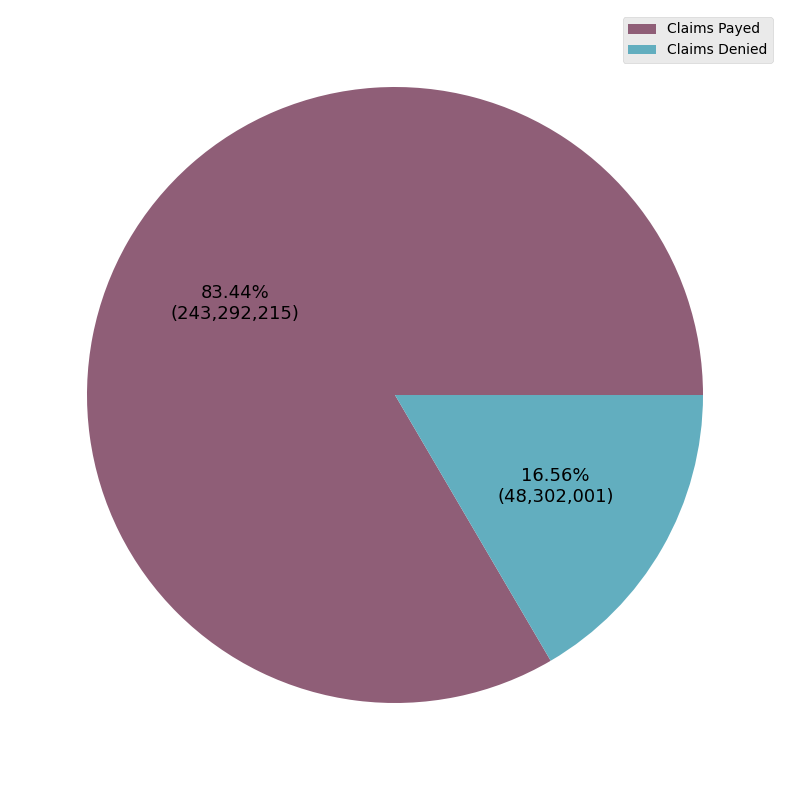
\includegraphics[width=.6\columnwidth]{images/cms_puf/overall_denial_pie.png}
				\caption{Aggregate denial rate across federal marketplace insurers in 2021. Approximately 16\% of all federal marketplace claims were initially denied in 2021, according to CMS TIC PUF data.}
				\label{federal_denial_rate}
			\end{figure}
		\clearpage
	
		\underline{New York Health Care Claims Reports}\\
		
			Among New York insurers, 18\% of all claims submitted in 2022 were initially denied. This data is displayed in Figure \ref{newyorkoveralldenial}.
			
			\begin{figure}[h!]
				\centering
				\textbf{Overall Claims Denial Rate, NY, 2022}\par\medskip
				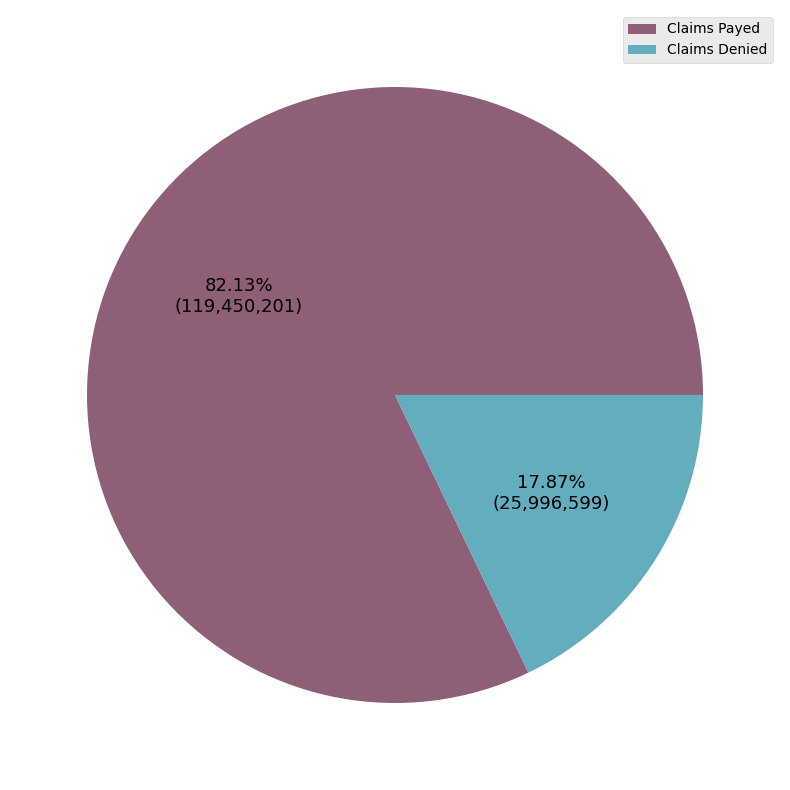
\includegraphics[width=.6\columnwidth]{images/ny_claim_reports/overall_denial_pie.png}
				\caption{Overall denial rate (18\%) among all NY issuers who submitted health care claims reports to the Department of Financial Services in 2022.}
				\label{newyorkoveralldenial}
			\end{figure}
		
		
		\underline{Connecticut Consumer Report Cards}\\
		
		Among Connecticut insurers, 25\% of all claims submitted in 2021 were initially denied. This calculation involved throwing out seemingly spurious data reported for the indemnity plans for one insurer, Connecticare (the report indicates Connecticare had more denials of claims than actual claims received). This data is displayed in Figure \ref{ctoveralldenial}.
		
		\begin{figure}[h!]
			\centering
			\textbf{Overall Claims Denial Rate, CT, 2021}\par\medskip
			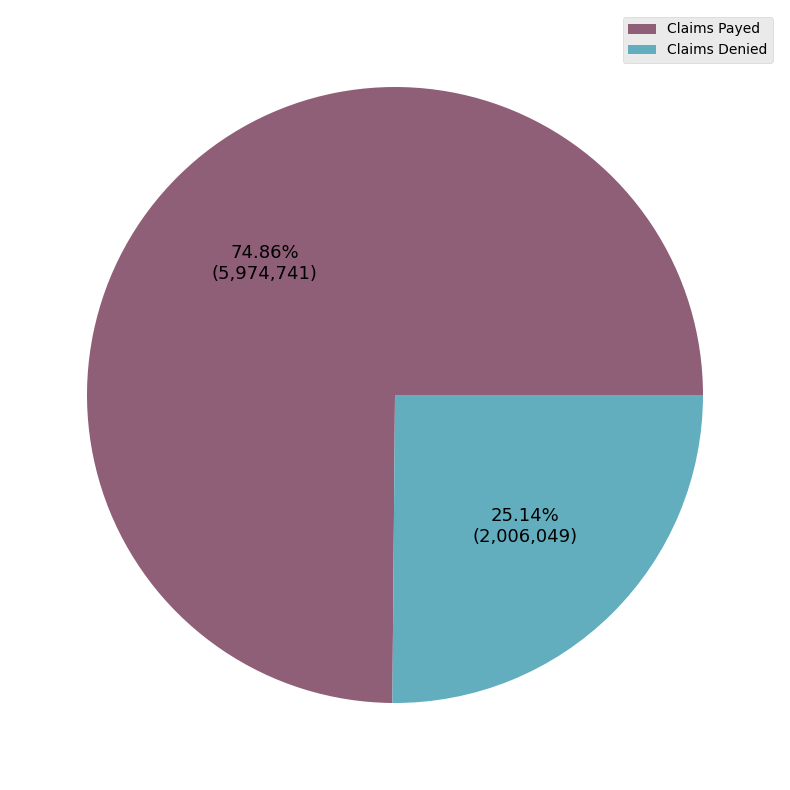
\includegraphics[width=.6\columnwidth]{images/ct_claims/overall_denial_pie.png}
			\caption{Overall claims denial rate in CT consumer report card data.}
			\label{ctoveralldenial}
		\end{figure}
		
		\underline{Pennsylvania Department of Insurance Data}\\
		
		Among Pennsylvania insurers represented in the PA DOI data, approximately 15\% of all claims submitted in 2020 were initially denied, while approximately 13\% of the claims submitted in 2021 were initially denied. This data is displayed in aggregate in Figure \ref{paoveralldenial}.
		
		\begin{figure}[h!]
			\centering
			\textbf{Overall Claims Denial Rate, PA, 2020-2021}\par\medskip
			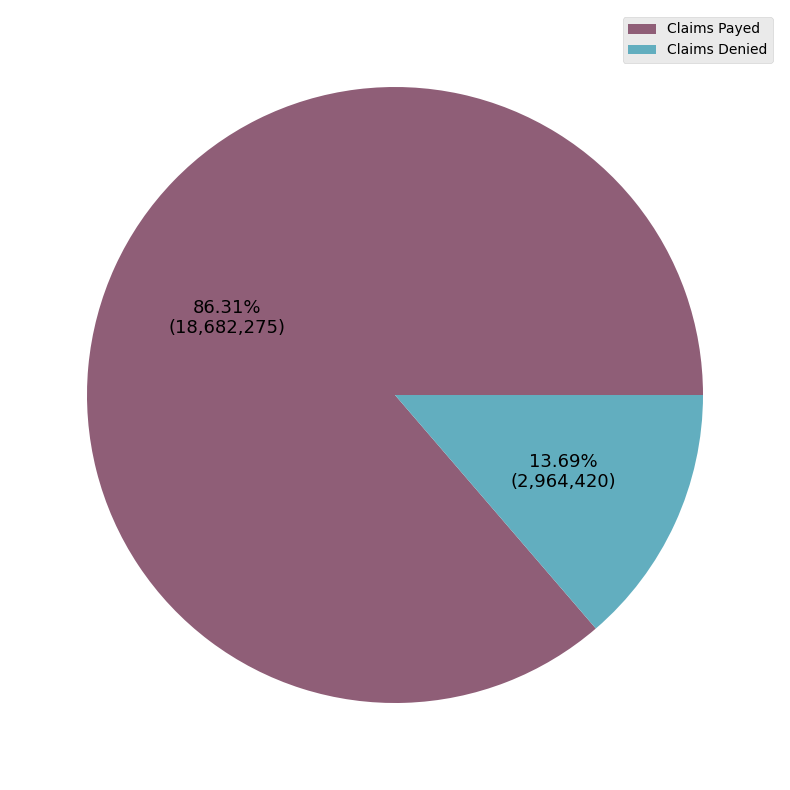
\includegraphics[width=.6\columnwidth]{images/pa_claims/overall_denial_pie.png}
			\caption{Overall claims denial rate in the Pennsylvania Department of Insurance data in 2020 and 2021.}
			\label{paoveralldenial}
		\end{figure}
		
		
		\subsubsection{Denials By Rationale}
		
		When insurers deny coverage of a claim, they must report their rationale for the denial. The rationales, and the details of how they must be reported to both the insured and regulatory agencies, vary by plan, but typically include a small set of mutually exclusive labels. In each of the datasets that provide denial counts, some metadata regarding the denial rationales is included, though the details vary by dataset.\\
		
		\underline{CMS Federal Marketplace PUFs}\\
		
		Federal marketplace plans included in the CMS TIC PUF data \emph{sometimes} report rationales for claim denials. Figure \ref{federalrationaledist} shows the categories allowed in the CMS PUF reporting methodology, and their frequency of occurrence in the subset of data which includes rationales.\\
		
		\begin{figure}[h!]
			\centering
			\textbf{Denials By Rationale, Federal Marketplace, 2021}\par\medskip
			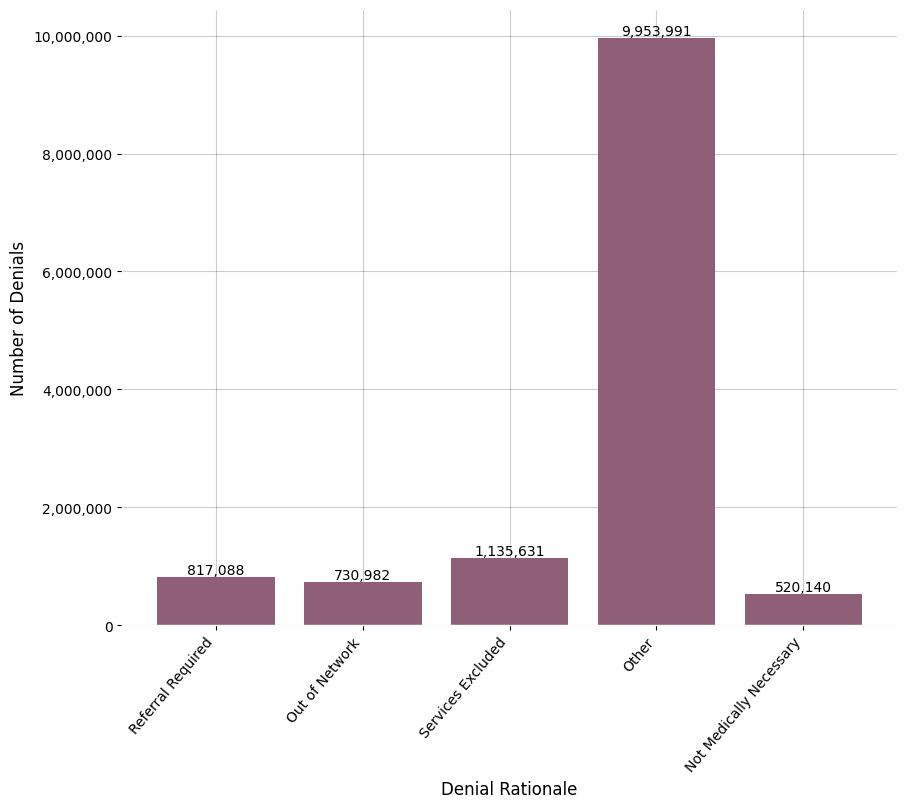
\includegraphics[width=\columnwidth]{images/cms_puf/denials_by_rationale.png}
			\caption{Distribution of claims denial rationales in a subset of the TIC PUF data. }
			\label{federalrationaledist}
		\end{figure}

		Most denials logged in the CMS PUF data are associated with a rationale of ``Other''. This provides little information about the underlying nature of the denials.\\
		
		Effectively, this reporting scheme allows insurers to withhold reporting the actual reason for a denial to the public if they so choose, since it is not completely clear what is allowed to be reported in the ``Other" bucket, and there is no strict validation of the reported data. Whether or not insurers actually abuse the system in this way cannot be gleaned from this data alone.\\
		
		\underline{New York Health Care Claims Reports}\\
		
		The New York Health Care Claims Reports detail the rationales for all of the denials documented in the data, but allow for a different set of available options for denial rationales. These rationales, and their relative frequency of occurrence within the data, are shown in Figure \ref{nyrationaledist}.\\ 
		
		\begin{figure}[h!]
			\centering
			\textbf{Denials By Rationale, NY, 2022}\par\medskip
			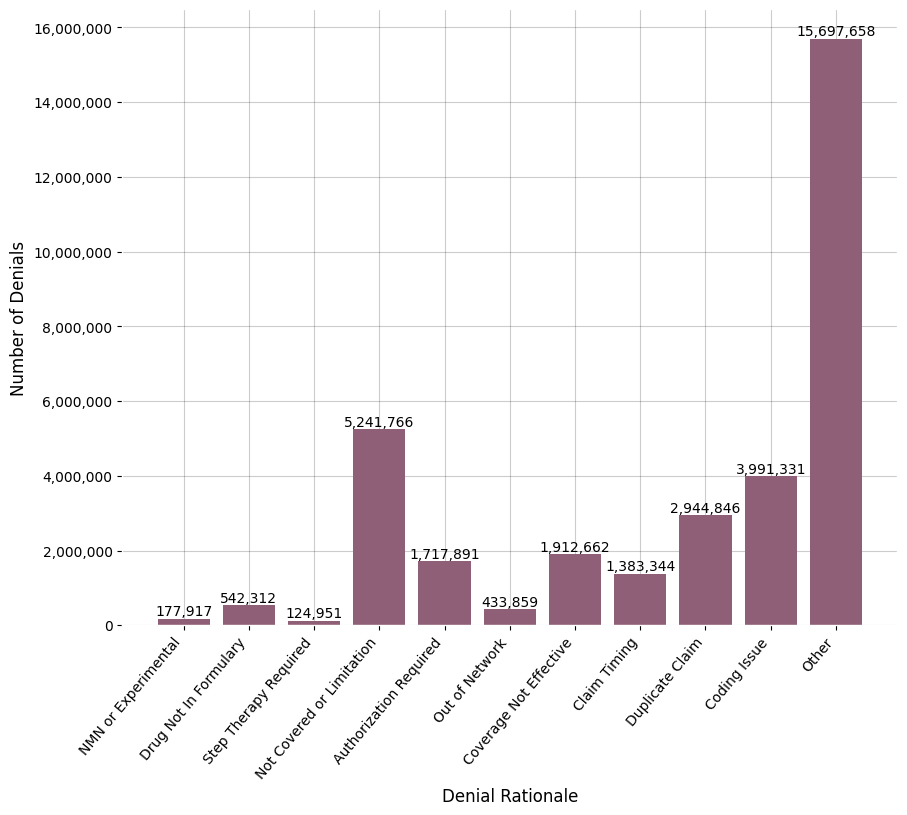
\includegraphics[width=\columnwidth]{images/ny_claim_reports/denial_rationale_dist.png}
			\caption{Distribution of denial rationales for all denials recorded in the health care claims reports submitted to the Department of Financial Services in 2022.}
			\label{nyrationaledist}
		\end{figure}
	
		Again, we see that an ambiguous "Other" category is utilized heavily in the reporting. Furthermore, while many of the rationale categories in this dataset are well-defined terms that have consistent, standard meaning across the industry (see e.g. a typical definition of \href{https://en.wikipedia.org/wiki/Step_therapy}{step therapy}), others are ambiguous.\\
		
		For example, the ``Not Covered or Limitation'' label here is our abbreviation of a label specified in the raw data as ``Not a covered benefit/Exceeds benefit limits (e.g., visit limits)'', which is a broad category that appears to allow for many interpretations, similar to the ``Other'' category. It would be useful to understand more explicitly exactly which subset of denials are being recorded in the ``Not Covered or Limitation'' category, as opposed to the ``Other'' category, or the ``NMN or Experimental'' category, since there is ambiguity and conceptual overlap in each of these concepts. For example, claims deemed to be not medically necessary or experimental are typically a subset of services that are explicitly considered ``not covered", according to language in insurance contracts.\\
		
		\underline{Connecticut Consumer Report Cards}\\
		
		The Connecticut consumer report cards detail rationales for every denial recorded in the data, but again use a different set of categories, and make liberal use of an "Other" category. The data is displayed in Figure \ref{ctrationaledist}.\\
		
		\begin{figure}[h!]
			\centering
			\textbf{Denials By Rationale, CT, 2021}\par\medskip
			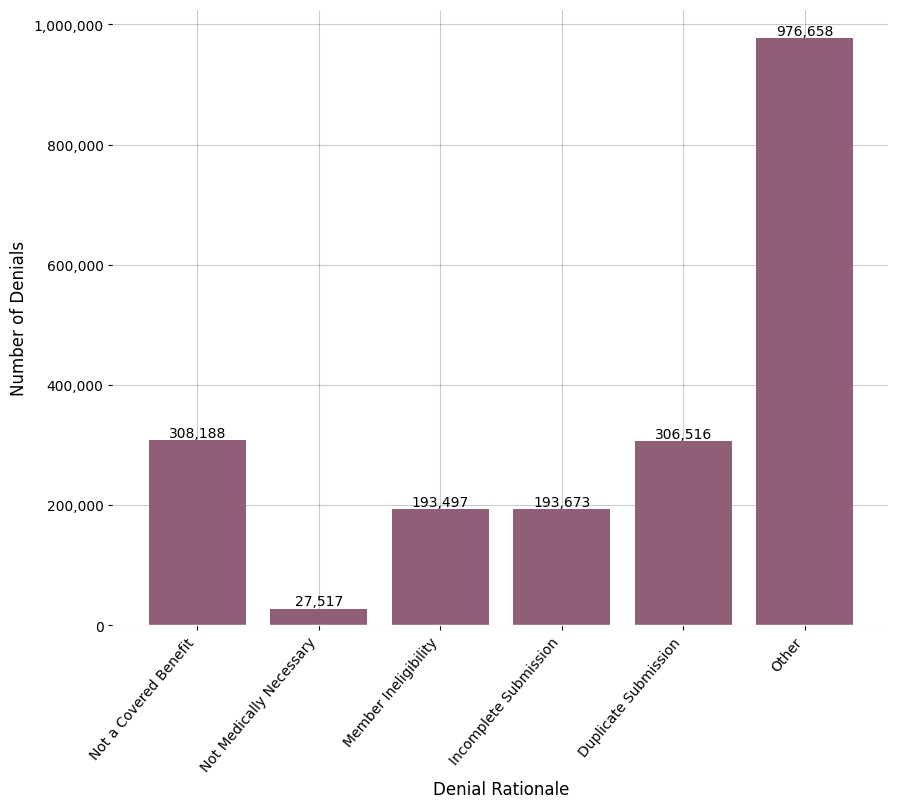
\includegraphics[width=\columnwidth]{images/ct_claims/denials_by_rationale.png}
			\caption{Distribution of denial rationales for all denials in the CT consumer report card data. }
			\label{ctrationaledist}
		\end{figure}
		
		\underline{Pennsylvania Department of Insurance Data}\\
		
		The Pennsylvania Department of Insurance data details rationales only for denials recorded at the plan level in the data (which is the subset corresponding to marketplace claims), but the story remains the same in that the set of permissible rationales in the data is distinct from each other set we've considered. The data is displayed in Figure \ref{parationaledist}.
		
		\begin{figure}[h!]
			\centering
			\textbf{Denials By Rationale, PA, 2020-2021}\par\medskip
			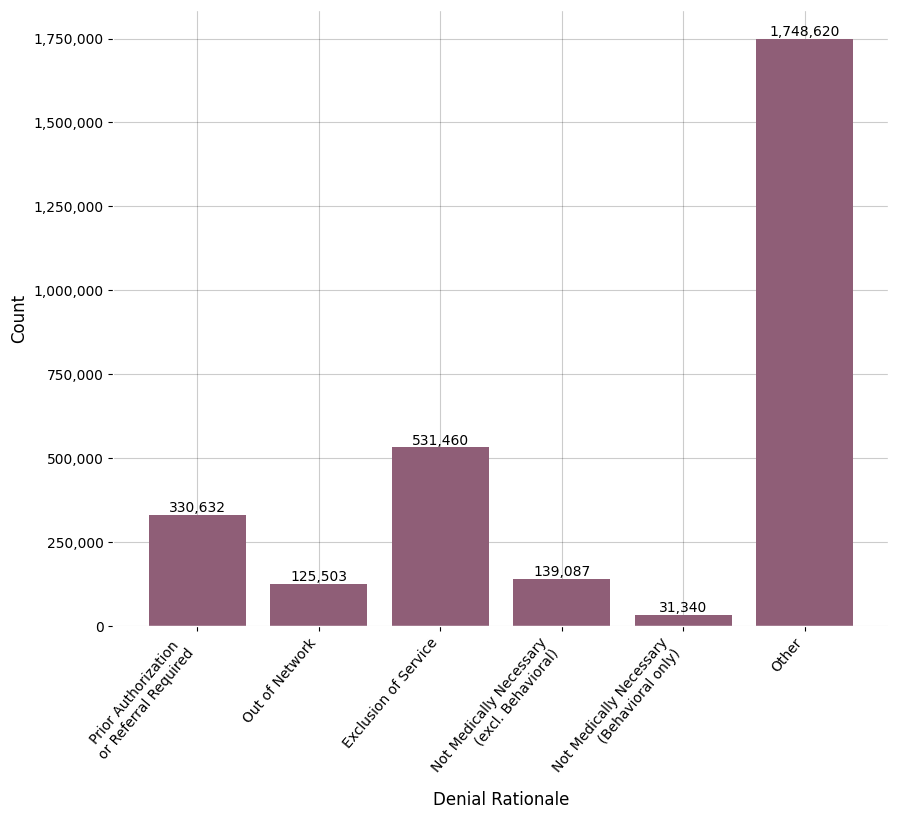
\includegraphics[width=\columnwidth]{images/pa_claims/denial_rationale_dist_2020-2021.png}
			\caption{Distribution of denial rationales for all denials in the PA DOI data.}
			\label{parationaledist}
		\end{figure}
		
		\subsubsection{`Not Medically Necessary' Denial Rates}
		
		Each of the datasets considered provides a category of denial rationale corresponding to purported lack of medical necessity or experimental nature of a service (what we will collectively call \emph{NMN denials}).\\
		
		While NMN denials occur \emph{relatively} infrequently, as Figures 5, 6, 7 and 8 show, they still correspond to a large population of claims in an absolute sense; just for the tiny fraction of all insurance plans covered by the data shown above, for a single plan year, there are more than 700k such claims. Furthermore, they are an important subset of denials in the sense that:\\
		
		\begin{itemize}
			\item Their contractual merit is typically subtle, because it typically involves contractual definitions that themselves reference things like clinical policy bulletins, scientific literature, medical standards, or other external data.
			\item The consequences for such denials can be perilous for patients relying on coverage of treatments for debilitating issues that they would not otherwise be able to afford. This can be true for other rationale categories as well, depending on the categories considered, but is not the case for all categories (e.g. duplicate claims).
		\end{itemize}
	
		For these reasons, we draw attention to aspects of the data pertaining specifically to NMN denials, when possible. Unfortunately, the data is often insufficient to allow much to be ascertained definitively about this subpopulation of denials.\\
		
		One thing we can understand definitively about the subpopulation of NMN denials in these datasets is the rate at which they occur among all claims; these rates can be deduced by reconsidering Figures \ref{federalrationaledist}, \ref{nyrationaledist}, \ref{ctrationaledist}, \ref{parationaledist} but we make the rates explicit in Table  \ref{nmndenialratetable} below.\\
		
		\begin{table}[!ht]
			\centering
			\begin{tabular}{|p{5cm}|p{3cm}|p{4cm}|p{3cm}|}
				\hline
				\textbf{Data Source} & \textbf{NMN Denials} & \textbf{Claims Received \newline With Rationale} & \textbf{NMN Denial \newline Rate}  \\ \hline
				CMS TIC PUF (2021) & 520,140 & 13,157,832 & .0395 \\ \hline
				NY Health Care Claims Reports (2022) & 177,881 & 34,168,504 & 	.0052 \\ \hline
				Connecticut Consumer Report Card (2021) & 27,517 & 2,006,049 &  .0137 \\ \hline
				Pennsylvania DOI Data (2020) & 104,396 & 10,451,280 &  .0099 \\ \hline
				Pennsylvania DOI Data (2021) & 66,031 & 	9,494,221 &  	.0069 \\ \hline
			\end{tabular}
			\caption{NMN Denial Rates}
			\label{nmndenialratetable}
		\end{table}
		
		
		Unsurprisingly we see that NMN denial rates are orders of magnitude smaller than overall denial rates; however, it is interesting to note that there is significant variation in the overall NMN denial rate across these datasets. One contributing factor is surely the lack of standardization in reporting methodologies, such as the variation in the set of denial rationales permissible in the reported data. It is unclear to what extent the actual denial rates relating to medical necessity would vary across these datasets if one were to correct for reporting inconsistencies. \\
		
		
		\subsubsection{Denials By Insurer}
		
		Each of the datasets reporting denials includes breakdowns of the claims received and claims denied by insurer. It is informative to understand how the aggregate denial rates and NMN denial rates vary by insurer within each dataset.
		
		We note at the outset that while it is informative to understand how various distributions vary by insurer, there are many subtleties lurking behind such breakdowns, just as there were for denial rationales. For example, different insurers may have different distributions of plan network types (e.g. relative fraction of consumers on HMO, EPO, PPO, and POS plans), and as a result insurer denial differences might partially be a reflection of the differences in those plan type distributions. Or, alternatively, two insurers might have identical plan type distributions and administration practices, but have a different list of drugs for which they require prior-authorization, with one list containing some much more commonly utilized drugs. Given such subtleties which the data does not allow us to address, it is difficult to definitively understand the cause of the phenomenology we observe in differences across insurers.
		
		In the same vein, the distribution across insurers of denials whose rationale specifically involves the experimental nature of a treatment, rather than another medical necessity rationale, could be influenced by many things, in addition to the raw counts of claims. In particular, one would expect that wealthy and renowned hospital systems conducting cutting edge research would be more likely than others to attempt truly experimental or novel services for their patients in need, and that such properties of a hospital are correlated with other properties, such as proximity to a major city and research center. As a result, health insurance companies with networks that overlap certain geographic areas, or that include certain hospitals, might receive a distribution of claims with a relatively high share that could be interpreted as involving experimental treatments, when compared to distributions received by other insurance companies. In such a context, it would be inappropriate to make an inference about how experimental claims denial processes vary by insurer from experimental claims denial rates alone.
		
		As with all of the data we examine in this article, there are many subtleties that make it difficult to draw conclusions without more information. We make suggestions to address this troubling predicament in a concluding policy section.

		
		\underline{CMS Federal Marketplace PUFs}\\
		
		Figures \ref{fedinsurerclaims}, \ref{fedinsurerdenialrates}, and \ref{fedinsurernmndenialrates} show the overall claims counts, denial rates, and NMN denial rates for the 10 issuers in the CMS TIC PUF Federal Marketplace data with the highest claims volume.
		
		
		\begin{figure}[h!]
			\centering
			\textbf{Claims Count By Insurer, Federal Marketplace, 2021}\par\medskip
			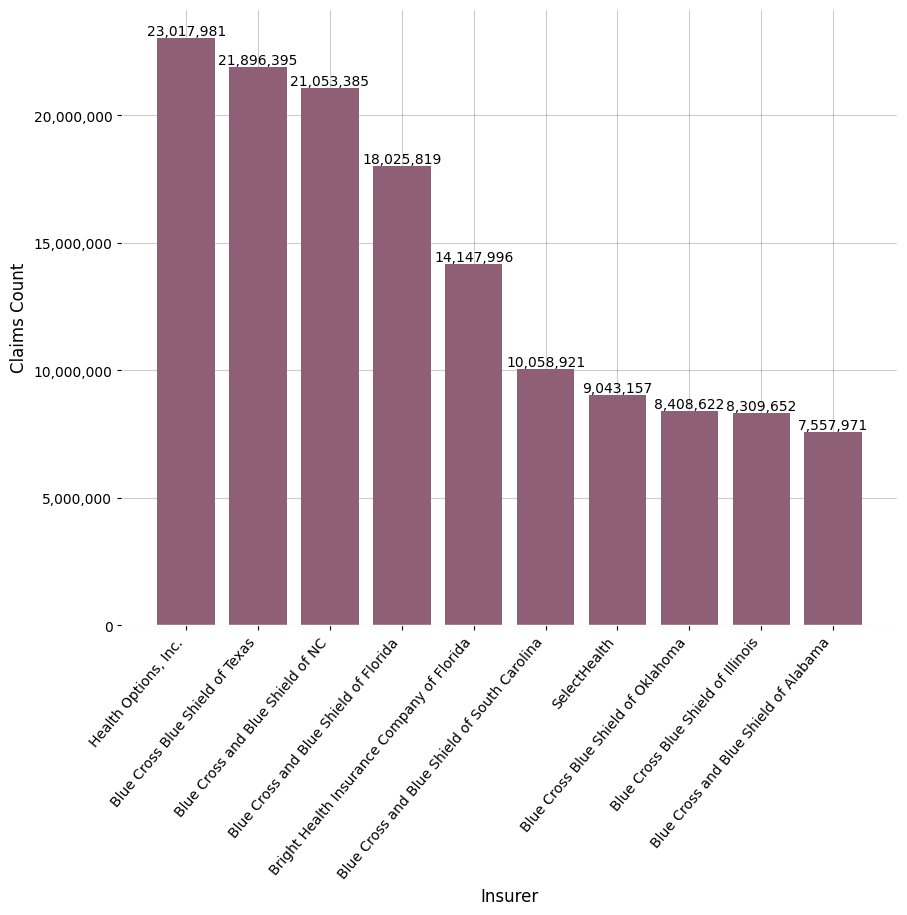
\includegraphics[width=\columnwidth]{images/cms_puf/claims_by_insurer.png}
			\caption{Claims received for the 10 issuers with the largest number of claims adjudicated in the 2021 CMS TIC PUF data.}
			\label{fedinsurerclaims}
		\end{figure}
	
		\clearpage
	
	
		\begin{figure}[h!]
			\centering
			\textbf{Denial Rate By Insurer, Federal Marketplace, 2021}\par\medskip
			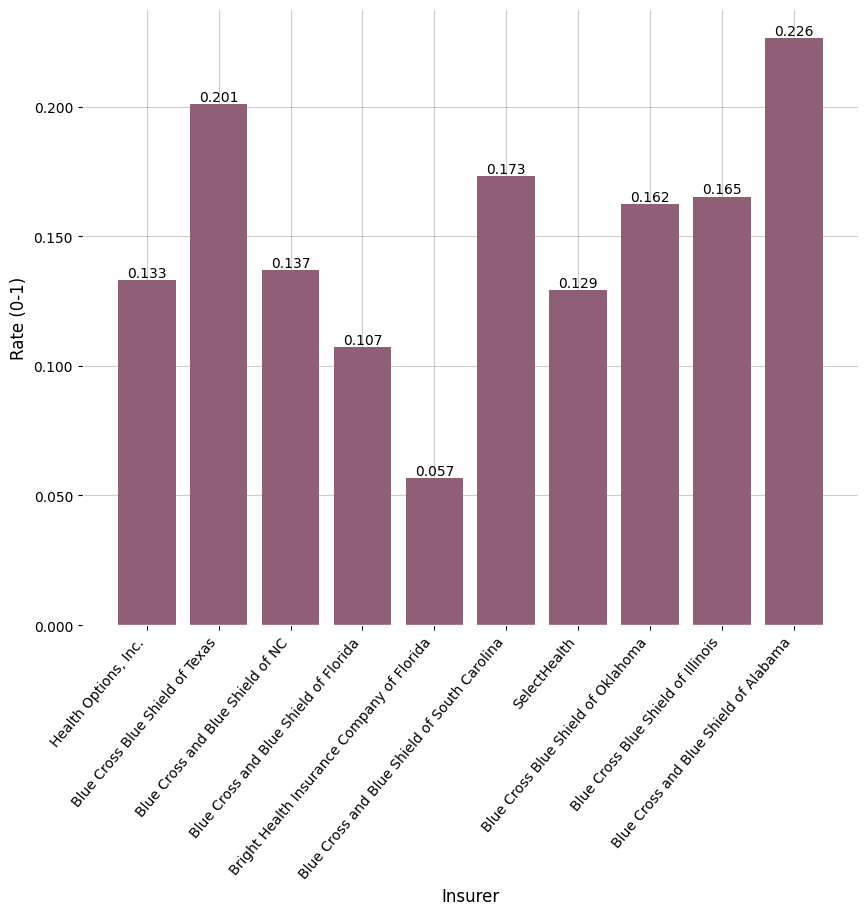
\includegraphics[width=\columnwidth]{images/cms_puf/denial_rate_by_insurer.png}
			\caption{Overall claims denial rates for the 10 issuers with the largest number of claims adjudicated in the 2021 CMS TIC PUF data.}
			\label{fedinsurerdenialrates}
		\end{figure}
	
		\clearpage
		
		\begin{figure}[h!]
			\centering
			\textbf{NMN Denial Rate By Insurer, Federal Marketplace, 2021}\par\medskip
			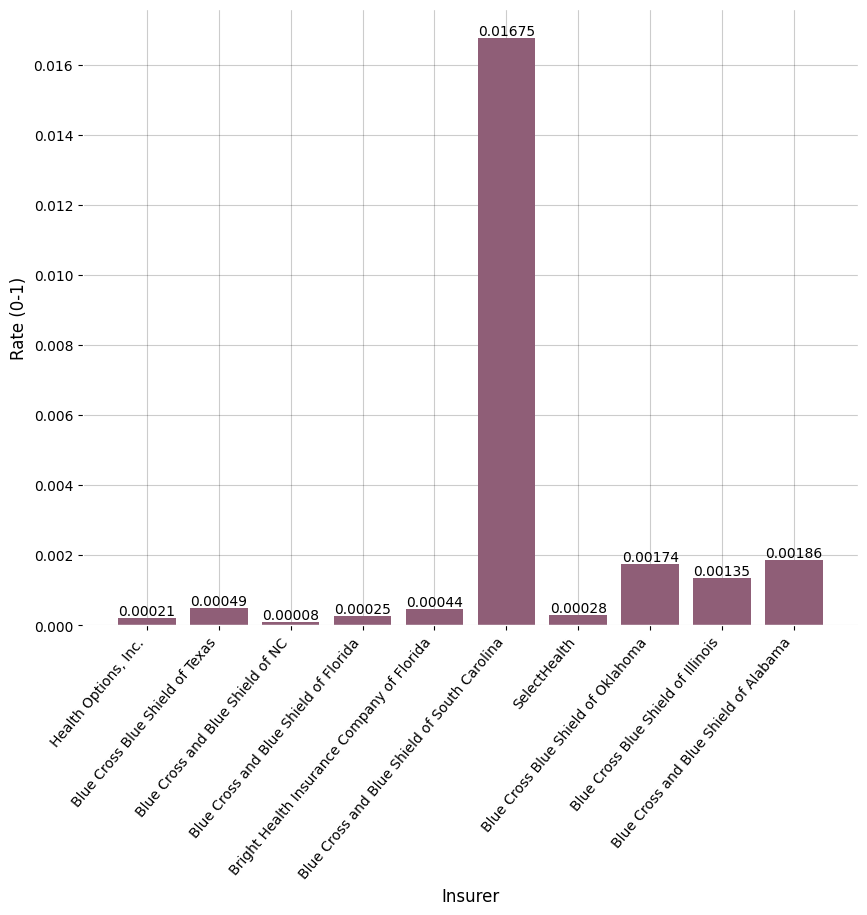
\includegraphics[width=\columnwidth]{images/cms_puf/nmn_denial_rate_by_insurer.png}
			\caption{NMN (including experimental) denial rates for the 10 issuers with the largest number of claims adjudicated in the 2021 CMS TIC PUF data.}
			\label{fedinsurernmndenialrates}
		\end{figure}
	
		Among the largest federal marketplace issuers of 2021, as measured by claims received, Blue Cross Blue Shield of South Carolina has an NMN denial rate roughly two to three orders of magnitude larger than the others. It is unclear what drives this phenomenon.
		
		Figure \ref{feddenialrationalesbyinsurer} shows a heatmap displaying the distribution of denial rationales among these same highest volume insurers.
		
		\begin{figure}[h!]
			\centering
			\textbf{Denial Rationales By Insurer, Federal Marketplace, 2021}\par\medskip
			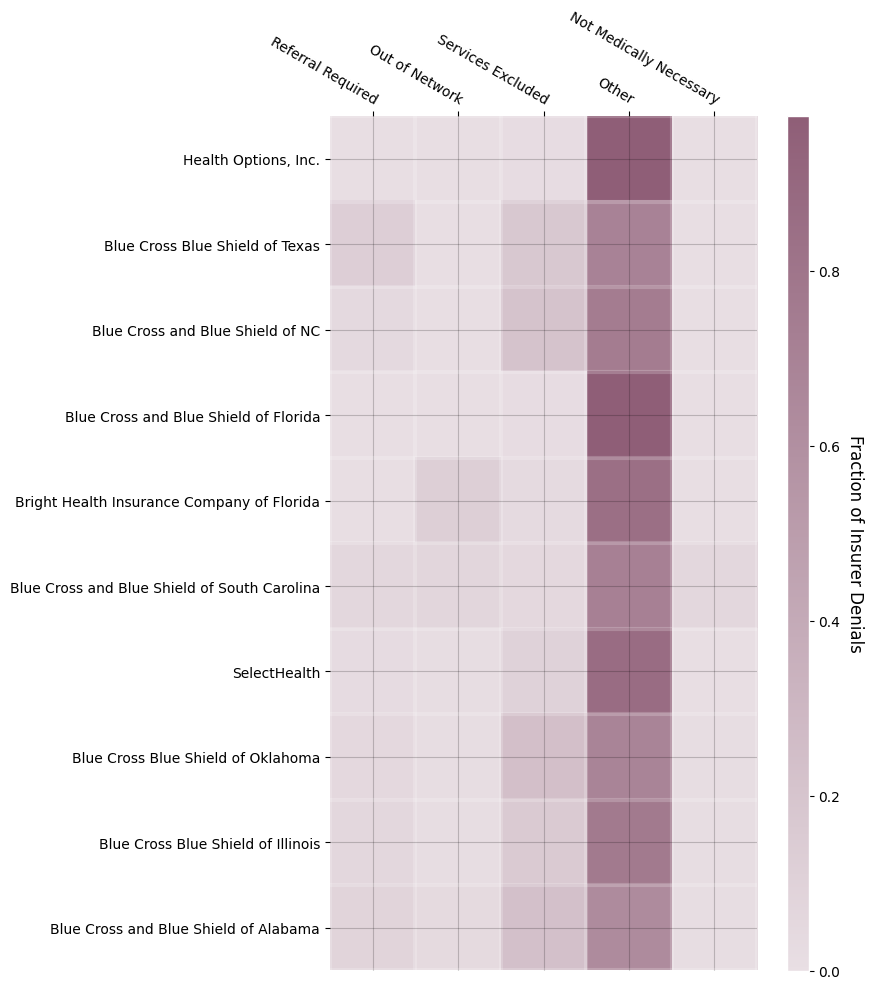
\includegraphics[width=\columnwidth]{images/cms_puf/insurer_vs_denial_cat.png}
			\caption{Distribution of denial rationales for the 10 issuers with the largest number of claims adjudicated in the 2021 CMS TIC PUF data. The color indicates the fraction of all denials for a given insurer that were coded with a particular rationale (i.e. rows sum to 1). }
			\label{feddenialrationalesbyinsurer}
		\end{figure}
	
		\clearpage
		
		
		
		\underline{New York Health Care Claims Reports}\\
		
				Figures \ref{nyinsurerclaims}, \ref{nyinsurerdenialrates}, and \ref{nyinsurernmndenialrates} show the overall claims counts, denial rates, and NMN denial rates for the 10 issuers in the New York Health Care Claims Reports data with the highest claims volume.
		
		\begin{figure}[h!]
			\centering
			\textbf{Claims Count By Insurer, NY, 2022}\par\medskip
			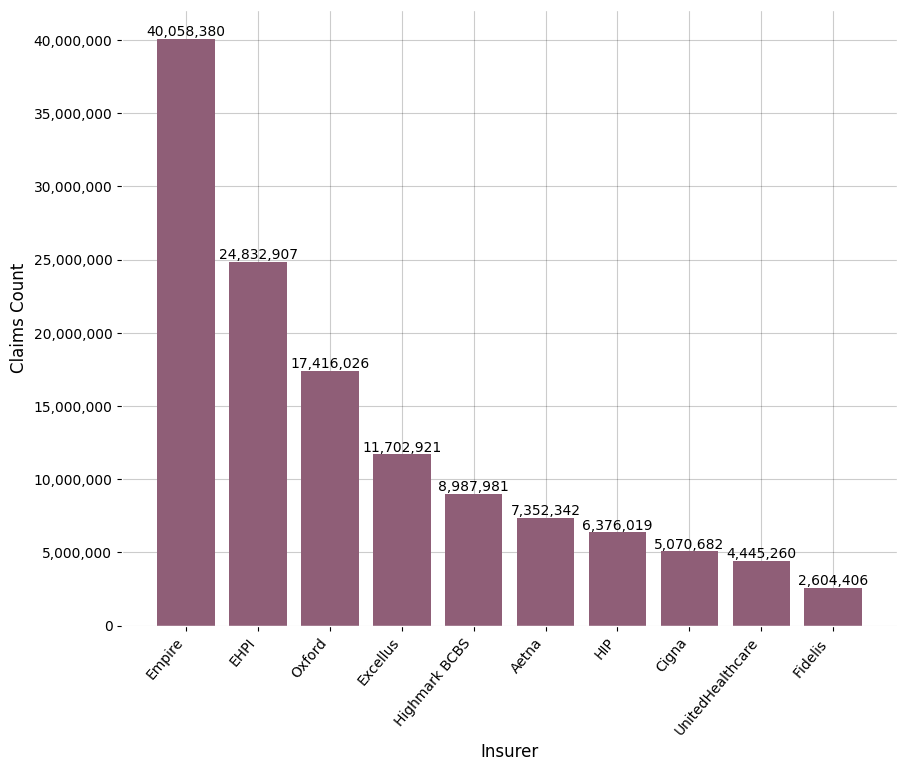
\includegraphics[width=\columnwidth]{images/ny_claim_reports/claims_by_insurer.png}
			\caption{Claims received for the 10 issuers with the largest number of claims adjudicated in the 2022 Department of Financial Services claims report data.}
			\label{nyinsurerclaims}
		\end{figure}
		
		\clearpage
		
		
		\begin{figure}[h!]
			\centering
			\textbf{Denial Rate By Insurer, NY, 2022}\par\medskip
			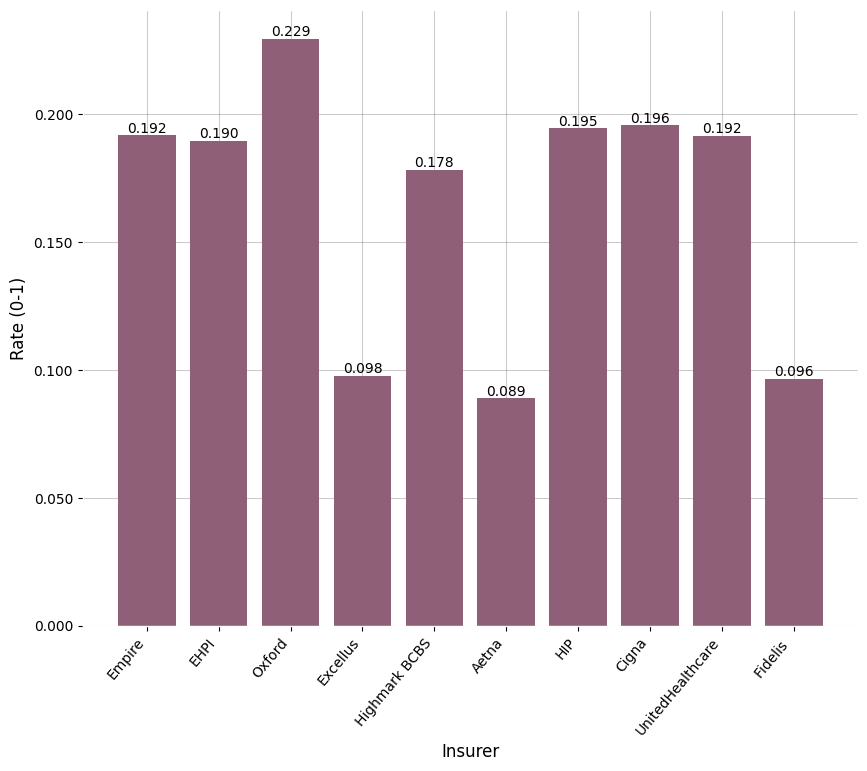
\includegraphics[width=\columnwidth]{images/ny_claim_reports/denial_rate_by_insurer.png}
			\caption{Overall claims denial rates for the 10 issuers with the largest number of claims adjudicated in the 2022 Department of Financial Services claims report data.}
			\label{nyinsurerdenialrates}
		\end{figure}
		
		\clearpage
		
		\begin{figure}[h!]
			\centering
			\textbf{NMN Denial Rate By Insurer, NY, 2022}\par\medskip
			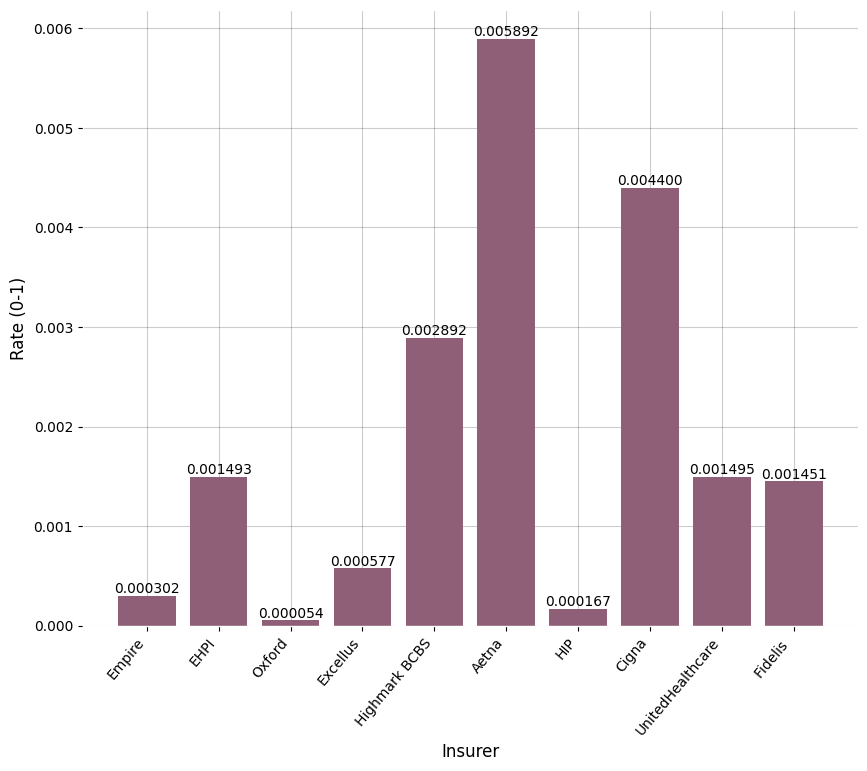
\includegraphics[width=\columnwidth]{images/ny_claim_reports/nmn_denial_rate_by_insurer.png}
			\caption{NMN (including experimental) denial rates for the 10 issuers with the largest number of claims adjudicated in the 2022 Department of Financial Services claims report data.}
			\label{nyinsurernmndenialrates}
		\end{figure}
	
		
		Figure \ref{nydenialrationalesbyinsurer} shows a heatmap displaying the distribution of denial rationales among these same highest volume insurers.
		
		\begin{figure}[h!]
			\centering
			\textbf{Denial Rationales By Insurer, NY, 2022}\par\medskip
			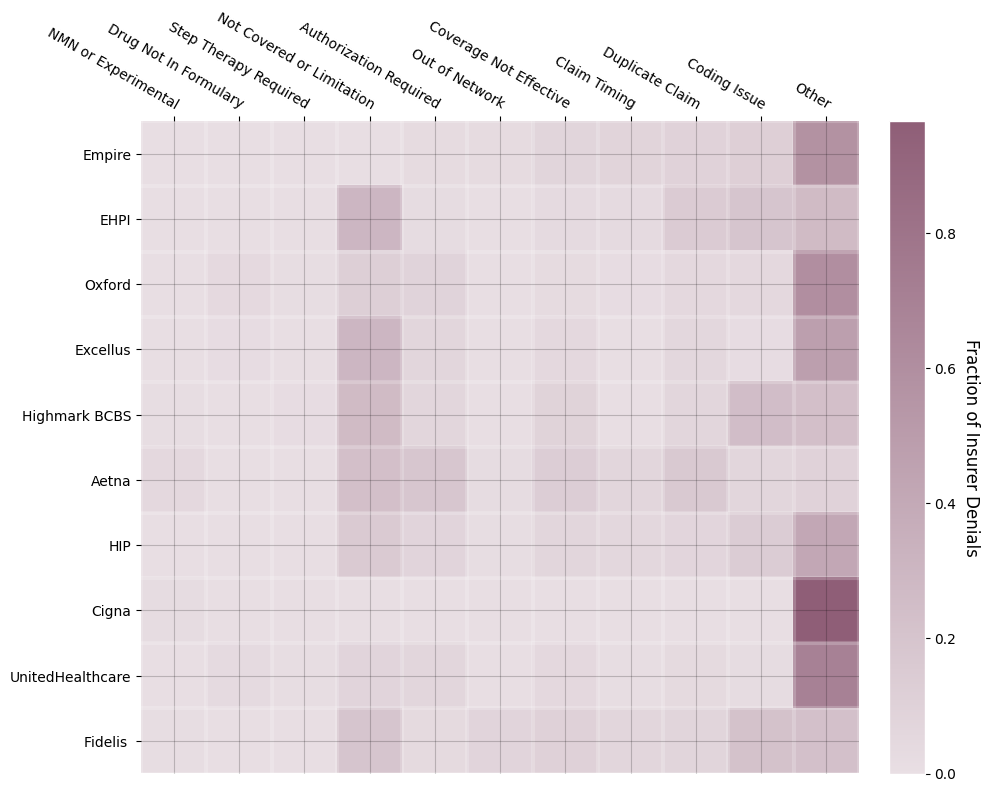
\includegraphics[width=\columnwidth]{images/ny_claim_reports/insurer_vs_denial_cat.png}
			\caption{Distribution of denial rationales for the 10 issuers with the largest number of claims adjudicated in the 2022 Department of Financial Services claims report data. The color indicates the fraction of all denials for a given insurer that were coded with a particular rationale (i.e. rows sum to 1).}
			\label{nydenialrationalesbyinsurer}
		\end{figure}
		
		\clearpage
		


		
		\underline{Connecticut Consumer Report Cards}\\
		
		
		Figures \ref{ctinsurerclaims}, \ref{ctinsurerdenialrates}, and \ref{ctinsurernmndenialrates} show the overall claims counts, denial rates, and NMN denial rates for the 10 issuers in the Connecticut Consumer Report Card data with the highest claims volume.

		\begin{figure}[h!]
			\centering
			\textbf{Claims Count By Insurer, CT, 2021}\par\medskip
			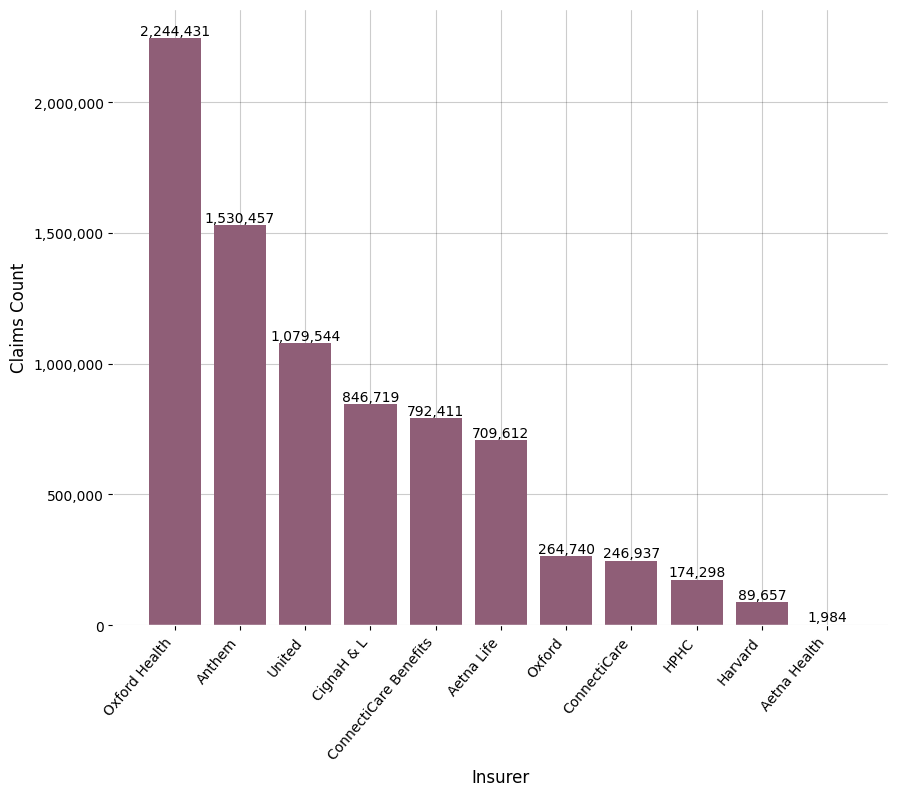
\includegraphics[width=\columnwidth]{images/ct_claims/claims_by_insurer.png}
			\caption{Claims received for all issuers in the CT consumer report card data.}
			\label{ctinsurerclaims}
		\end{figure}
		
		\clearpage
		
		
		\begin{figure}[h!]
			\centering
			\textbf{Denial Rate By Insurer, CT, 2021}\par\medskip
			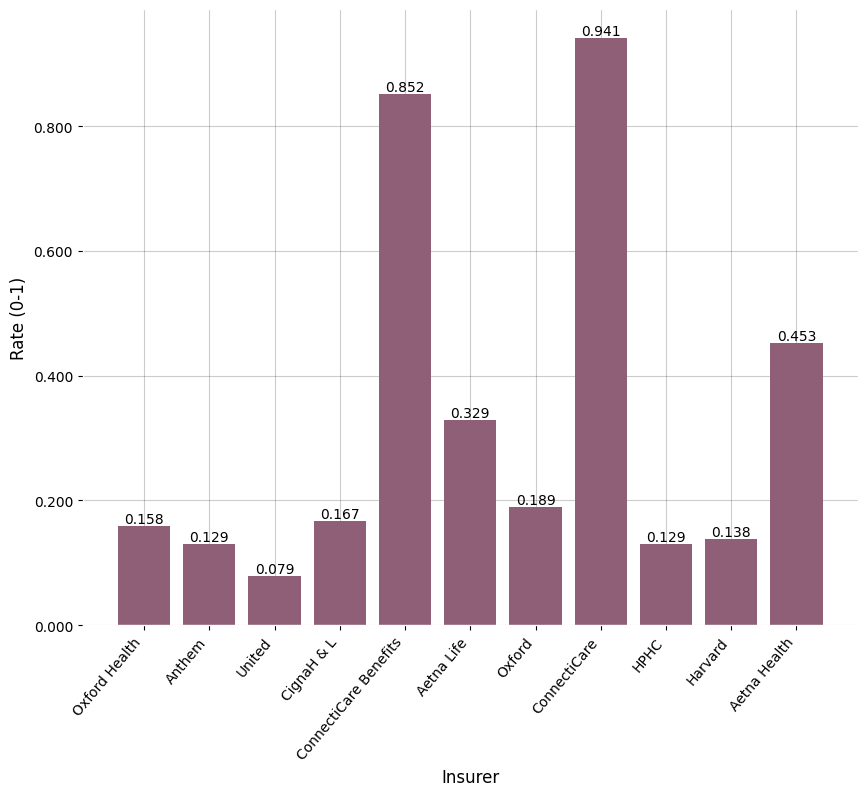
\includegraphics[width=\columnwidth]{images/ct_claims/denial_rate_by_insurer.png}
			\caption{Overall claims denial rates for all issuers in the CT consumer report card data.}
			\label{ctinsurerdenialrates}
		\end{figure}
		
		\clearpage
		
		\begin{figure}[h!]
			\centering
			\textbf{NMN Denial Rate By Insurer, CT, 2021}\par\medskip
			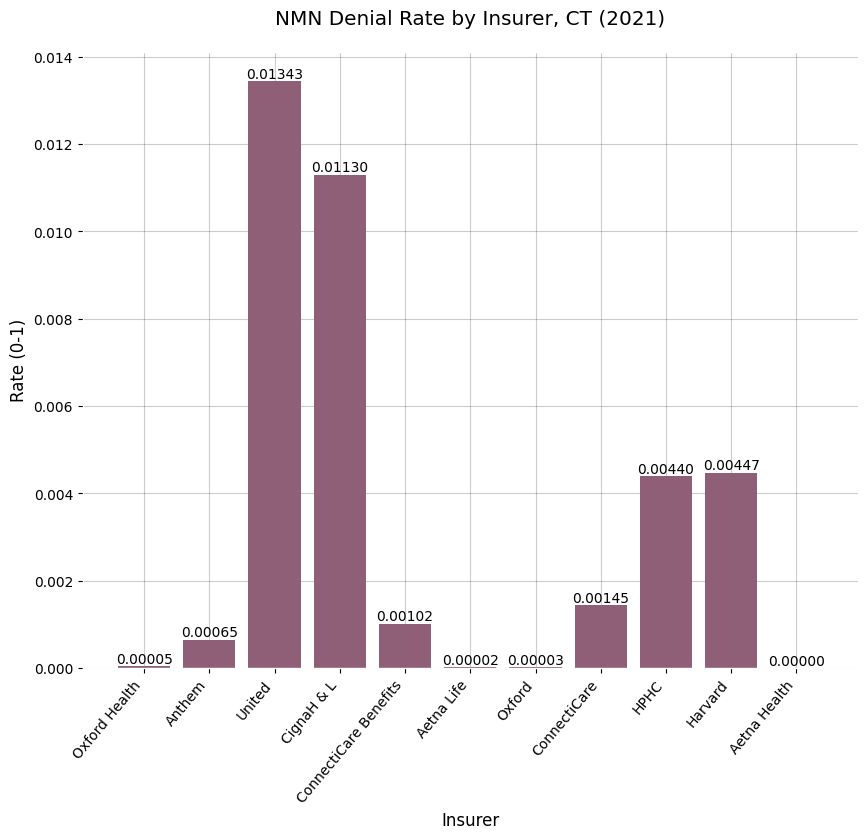
\includegraphics[width=\columnwidth]{images/ct_claims/nmn_denial_rate_by_insurer.png}
			\caption{NMN (including experimental) denial rates for all issuers in the CT consumer report card data.}
			\label{ctinsurernmndenialrates}
		\end{figure}
	
		Figure \ref{ctinsurerdenialrates} shows odd and potentially spurious data that indicates one set of issuers, 'ConnectiCare Benefits' and 'ConnectiCare', have extremely high claims denial rates above 85\%. We suspect this is a reporting error in the raw data, but we show it here because we cannot be sure of that fact. We were unable to find further information about this anomaly.
		
		Figure \ref{ctdenialrationalesbyinsurer} shows a heatmap displaying the distribution of denial rationales among these same highest volume insurers.

		
		\begin{figure}[h!]
			\centering
			\textbf{Denial Rationales By Insurer, CT, 2021}\par\medskip
			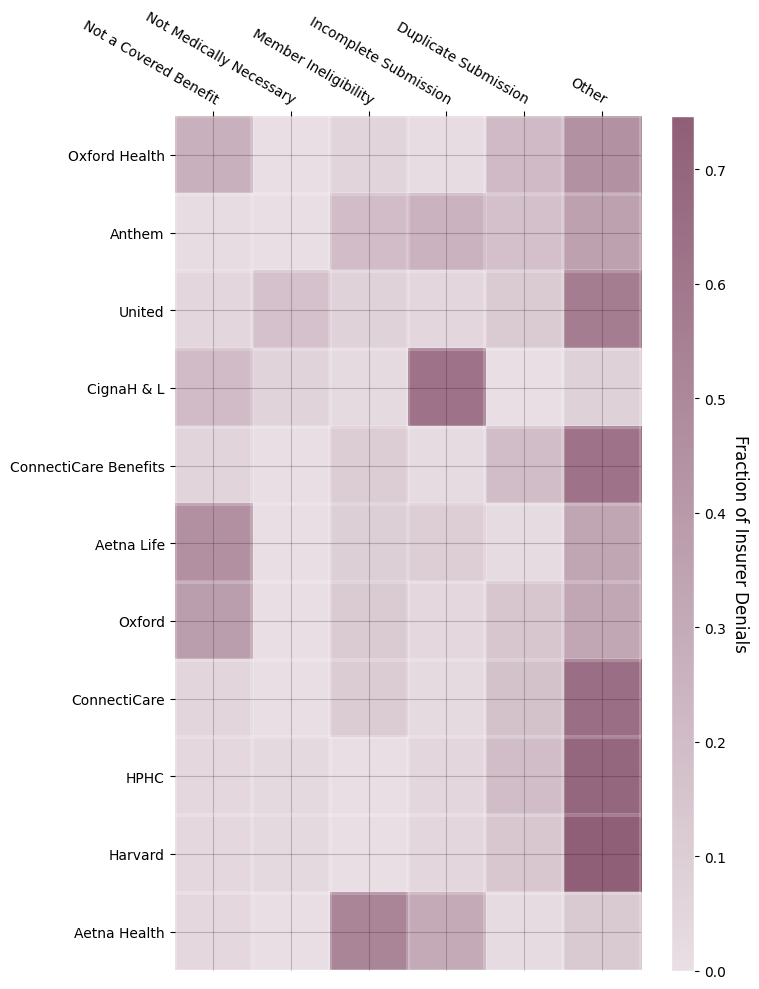
\includegraphics[width=\columnwidth]{images/ct_claims/insurer_vs_denial_cat.png}
			\caption{Distribution of denial rationales for all issuers in the CT consumer report card data. The color indicates the fraction of all denials for a given insurer that were coded with a particular rationale (i.e. rows sum to 1).}
			\label{ctdenialrationalesbyinsurer}
		\end{figure}
		
		\clearpage
		
		
		\underline{Pennsylvania Department of Insurance Data} \\
		
		
		Figures \ref{painsurerclaims}, \ref{painsurerdenialrates}, and \ref{painsurernmndenialrates} show the overall claims counts, denial rates, and NMN denial rates for the 10 issuers in the Pennsylvania Department of Insurance Data data with the highest claims volume.
	

		\begin{figure}[h!]
			\centering
			\textbf{Claims Count By Insurer, PA, 2020-2021}\par\medskip
			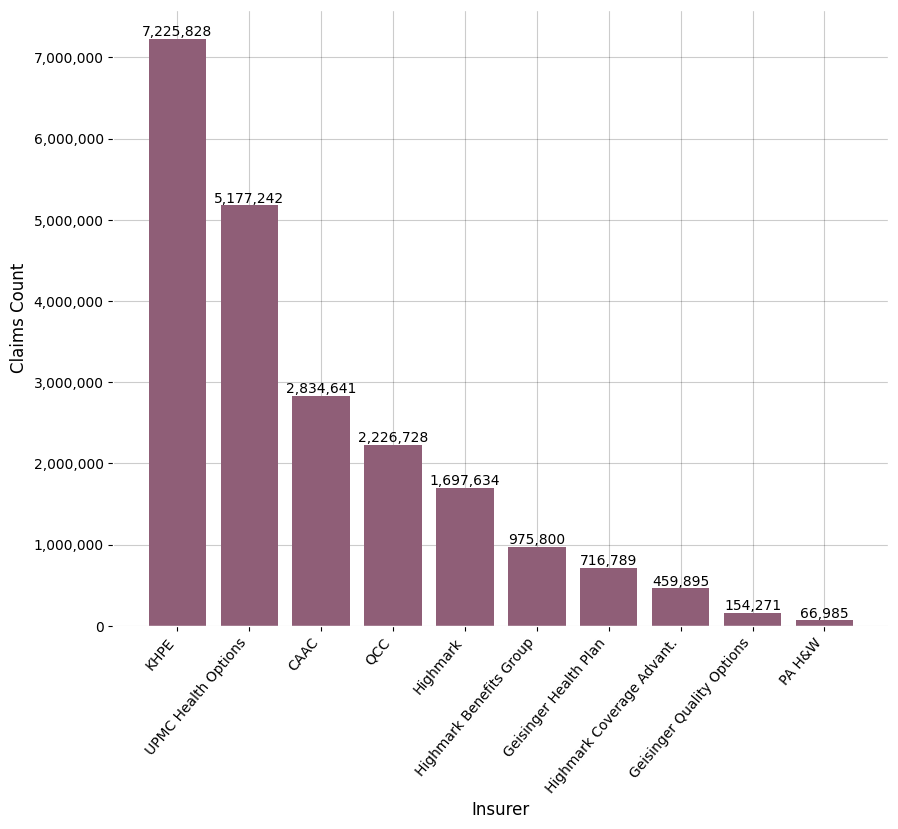
\includegraphics[width=\columnwidth]{images/pa_claims/claims_by_insurer.png}
			\caption{Claims received for all issuers in the PA DOI data.}
			\label{painsurerclaims}
		\end{figure}
		
		\clearpage
		
		
		\begin{figure}[h!]
			\centering
			\textbf{Denial Rate By Insurer, PA, 2020-2021}\par\medskip
			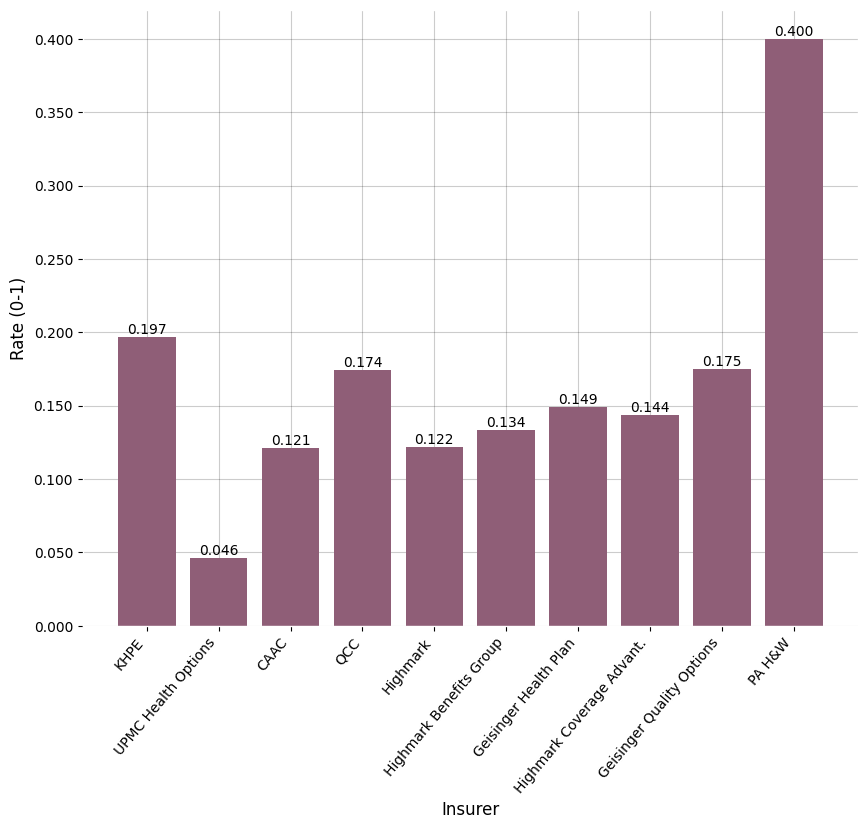
\includegraphics[width=\columnwidth]{images/pa_claims/denial_rate_by_insurer.png}
			\caption{Overall claims denial rates for all issuers in the PA DOI data.}
			\label{painsurerdenialrates}
		\end{figure}
		
		\clearpage
		
		\begin{figure}[h!]
			\centering
			\textbf{NMN Denial Rate By Insurer, PA, 2020-2021}\par\medskip
			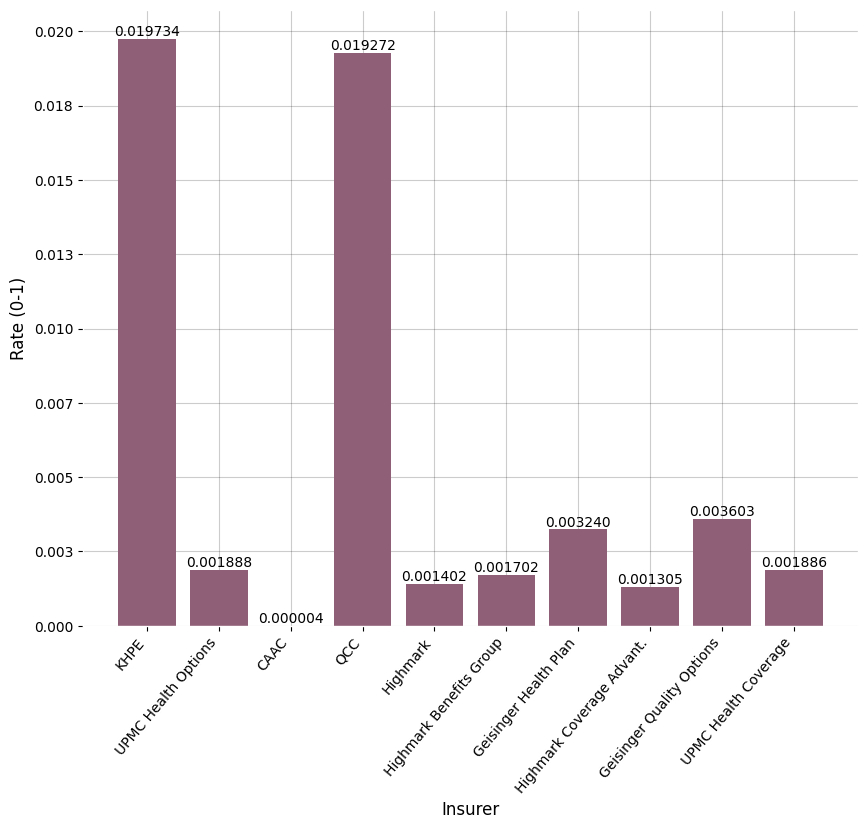
\includegraphics[width=\columnwidth]{images/pa_claims/nmn_denial_rate_by_insurer.png}
			\caption{NMN (including experimental) denial rates for all issuers in the PA DOI data.}
			\label{painsurernmndenialrates}
		\end{figure}
		
		
		Figure \ref{psdenialrationalesbyinsurer} shows a heatmap displaying the distribution of denial rationales among these same highest volume insurers.
		
		
		\begin{figure}[h!]
			\centering
			\textbf{Denial Rationales By Insurer, PA, 2020-2021}\par\medskip

			\caption{Distribution of denial rationales for all issuers in the PA DOI data who report denial rationales. The color indicates the fraction of all denials for a given insurer that were coded with a particular rationale (i.e. rows sum to 1).}
			\label{padenialrationalesbyinsurer}
		\end{figure}
		
		\clearpage
		
		
		
		
		\subsubsection{Dataset Specific Considerations}
		
		Since the datasets do not report claims and denial information in a standard or consistent way, there are many interesting considerations that can be made for only some of the datasets. Here we present dataset specific considerations relating to claims and denial distributions.
		
		
		
		\underline{CMS Federal Marketplace PUFs}\\
		
		The CMS TIC PUFs provide many pieces of metadata associated with individual plans, and their corresponding aggregate claims data, that allow denials to be broken down across additional categories.
		
		At a high level, we can calculate the overall denial rate for each \emph{issuer} (an insurer's \href{https://www.law.cornell.edu/definitions/uscode.php?width=840&height=800&iframe=true&def_id=26-USC-392827901-289353966&term_occur=1&term_src=}{state specific entity)}, by calculating the ratio of all claims denied by that issuer, to the claims received by that issuer (across all their plans). Figure 25 shows the distribution of such issuer denial rates across issuers represented in the 2021 CMS TIC PUF data. The distribution is bimodal, with a large majority of issuers comprising a contingency with aggregate denial rates between 0\% to 30\%, and a small contingency of issuers maintaining aggregate denial rates between 35\% to 50\%. While we could compute such a distribution for the other datasets as well, the number of issuers involved is too small to infer much from the resulting distribution. Here, however, the distribution sheds some light on how denial rates vary by issuer.
		
		
		\underline{New York Health Care Claims Reports}\\
		
		\underline{Connecticut Consumer Report Cards}\\
		
		\underline{Pennsylvania Department of Insurance Data}
		
		
		\subsection{Internal Appeals}\label{publicdata:internalappeals}
		
		
		\subsubsection{Overall Internal Appeal Rates}
		
		\subsubsection{Internal Appeals By Insurer}
		
		\subsubsection{Dataset Specific Considerations}
		
		\subsection{External Appeals}\label{publicdata:externalappeals}
		
		\subsubsection{Overall External Appeal Rates}
		
		\subsubsection{External Appeals By Denial Rationale}
		
		\subsubsection{External Appeal Overturn Rates Over Time}
		
		\subsubsection{External Appeals Overturn Rates By Insurer}
		
		\subsubsection{External Appeal Overturn Rates By Independent Review Organization}
		
		\subsubsection{External Appeal Overturn Rates By Underlying Medical Characteristics}
		
		\chapter{Conclusions}\label{conclusions}
		
		\subsection{Bias and Lack of Evaluation in Internal Appeal Processes}
		
		\subsection{Monetary Value of Appeals}
		
		\subsection{Need for Data Standardization, Validation and Enhancement}
		
		\subsection{Need for Standardization and Streamlining of Appeals Processes}
		
		\chapter{Recommendations}\label{recommendations}
		
		\subsection{Policy}
		
		\subsubsection{Disallow Requirements For Internal Appeals}
		
		\subsubsection{Levy Insurer Fines For External Appeal Overturns}
		
		\subsubsection{Mandate Transparent, Standardized Data Reporting For Denials and Appeals Across All Plans}
		
		\subsubsection{Mandate Transparent, Standardized Processes and Forms for Appeals Across All Plans}
		
		\subsection{Patient Recourse}
		
		\subsubsection{Appeal}
		
		\subsubsection{Contact Regulators}
		
		\subsubsection{Contact Our Team For Help}
		
		\subsubsection{Share Your Stories}
		
		\chapter{Reproducibility Statement}\label{reproducibilitystatement}
		
		
		\chapter{Acknowledgments}
		It is a pleasure to thank the following people for their support and guidance in reviewing this manuscript:
		
		
		
		\bibliographystyle{alpha}
		\bibliography{References}
		
		
	\end{document}